\documentclass[pdftex,12pt,a4paper]{article}

\input{/home/boris/science/tex_general/title_bor_utf8}


\providecommand{\indef}[1]{\textbf{#1}}


\usepackage{chessboard} % для рисования шахматной доски в одной из задач
% yum install texlive-chessboard texlive-skaknew


\begin{document}
\parindent=0 pt % отступ равен 0


% это магическое заклинание направляющее ребра к центру узла, а не к точке под узлом
\tikzset{edge from parent/.style=
     {draw, edge from parent path={(\tikzparentnode) -- (\tikzchildnode)}}}


% конвенция:
% при прочих равных названия ходов на дереве - маленькими буквами
% исключения - слова In, Out, ...



%\section{Методические рекомендации для преподавателей и студентов при проведении семинарских занятий по курсу теории игр ГУ-ВШЭ}

%\newpage

\section{Матричная форма, осторожные стратегии, обратная индукция (начало)}

$[$Slantchev$]$ - глава Elements of basic models, $[$IGT$]$ - глава 2,5 \\

\small
Информационное множество\footnote{Версия от \today, \url{http://pokrovka11.wordpress.com/} } --- один или несколько узлов, которые игрок не может различить между собой (пунктир на дереве) \\
Стратегия --- инструкция, указывающая какой ход нужно выбирать в каждом узле (информационном множестве). Стратегия позволяет игроку продолжить игру с любой позиции, не только с начальной. \\
Профиль стратегий или исход --- набор стратегий по одной от каждого игрока \\
Игра с совершенной информацией --- игра, где каждый игрок знает всю предысторию игры;  на дереве есть только одноточечные информационные множества\\
Осторожная стратегия --- стратегия, которую выберет игрок, предполагающий, что при любом его выборе для него произойдет самое худшее\\
Антагонистическая игра --- игра двух игроков, в которой выигрыш одного игрока равен проигрышу другого\\
Природа или Случай --- особый игрок, у которого изначально заданы вероятности ходов (буква N на дереве).\\
Суть метода обратной индукции --- начиная с конца игры определяем, кому как выгодно пойти. Каждый игрок выбирает больший средний выигрыш. Применим в играх с совершенной информацией. \\
\normalsize

\begin{enumerate}
\item В саду растут деревья...


\begin{tikzpicture}[grow=down] % дерево
\tikzstyle{mystart} = [circle, minimum width=3pt,fill, inner sep=0pt] % starting node style
\tikzstyle{mydot} = [circle, minimum width=2pt,fill, inner sep=0pt] % decision node style
\tikzstyle{level 1}=[sibling distance=2cm] % расстояние между соседними узлами на одном уровне
\tikzstyle{level 2}=[sibling distance=2cm]
\tikzstyle{level 3}=[sibling distance=2cm]
\node[mystart, label=above: {I}] {} % создаем узел типа mydot, с пометкой "N" сверху и пустым текстом внутри узла
    child { node[mydot, label=below: {$-1,1$}] {}        
    edge from parent node[left] {$l$} }
    child { node[mydot, label=above: {II} ] {}        
        child { node[mydot, label=below: {$4,4$}] {} 
        edge from parent node[left] {$c$} }
        child { node[mydot, label=above: {I}] (b) {}
                	child {	node[mydot, label=below: {$1,5$}] {}
                	edge from parent node[left] {$x$}}
                	child {	node[mydot, label=below: {$0,7$}] {}
                	edge from parent node[right] {$y$}  }
        edge from parent node[right] {$d$} }
    edge from parent node[right] {$r$} };
\end{tikzpicture}



\begin{tikzpicture}[grow=down] % дерево
\tikzstyle{mystart} = [circle, minimum width=3pt,fill, inner sep=0pt] % starting node style
\tikzstyle{mydot} = [circle, minimum width=2pt,fill, inner sep=0pt] % decision node style
\tikzstyle{level 1}=[sibling distance=4cm] % расстояние между соседними узлами на одном уровне
\tikzstyle{level 2}=[sibling distance=2cm]
\tikzstyle{level 3}=[sibling distance=2cm]
\node[mystart, label=above: {I}] {} % создаем узел типа mydot, с пометкой "N" сверху и пустым текстом внутри узла
    child { node[mydot, label=above: {II}] {}
    	child { node[mydot, label=below: {$3,2$}] {} 
		edge from parent node[left] {$a$} }        
    	child {	node[mydot, label=below: {$-1,-1$}] {} 
		edge from parent node[right] {$b$} } 
    edge from parent node[left] {$l$} }
    child { node[mydot, label=above: {II} ] {}        
        child { node[mydot, label=below: {$4,4$}] {} 
        edge from parent node[left] {$c$} }
        child { node[mydot, label=above: {I}] (b) {}
        	child { node[mydot, label=below: {$1,5$}] {}
            edge from parent node[left] {$x$}}
            child {	node[mydot, label=below: {$0,7$}] {}
            edge from parent node[right] {$y$}  }
        edge from parent node[right] {$d$} }
    edge from parent node[right] {$r$} };
\end{tikzpicture}

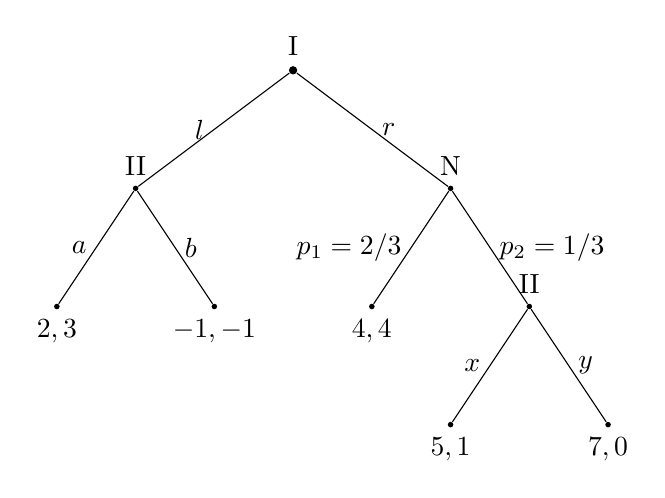
\begin{tikzpicture}[grow=down] % дерево
\tikzstyle{mystart} = [circle, minimum width=3pt,fill, inner sep=0pt] % starting node style
\tikzstyle{mydot} = [circle, minimum width=2pt,fill, inner sep=0pt] % decision node style
\tikzstyle{level 1}=[sibling distance=4cm] % расстояние между соседними узлами на одном уровне
\tikzstyle{level 2}=[sibling distance=2cm]
\tikzstyle{level 3}=[sibling distance=2cm]
\node[mystart, label=above: {I}] {} % создаем узел типа mydot, с пометкой "N" сверху и пустым текстом внутри узла
    child { node[mydot, label=above: {II}] {}
    	child { node[mydot, label=below: {$2,3$}] {} 
		edge from parent node[left] {$a$} }        
    	child {	node[mydot, label=below: {$-1,-1$}] {} 
		edge from parent node[right] {$b$} } 
    edge from parent node[left] {$l$} }
    child { node[mydot, label=above: {N} ] {}        
        child { node[mydot, label=below: {$4,4$}] {} 
        edge from parent node[left] {$p_1=2/3$} }
        child { node[mydot, label=above: {II}] (b) {}
                child { node[mydot, label=below: {$5,1$}] {}
              	edge from parent node[left] {$x$}}
                child { node[mydot, label=below: {$7,0$}] {}
               	edge from parent node[right] {$y$}  }
        edge from parent node[right] {$p_2=1/3$} }
    edge from parent node[right] {$r$} };
\end{tikzpicture}

\begin{enumerate}
\item Сколько стратегий у каждого игрока? Сколько в игре исходов?
\item Выпишите все профили стратегий, при которых, игра оканчивается в узле (-1;-1).
\item Переведите игру в матричную форму
\item Решите игру методом обратной индукции 
\end{enumerate}

\item В лесу растут деревья...



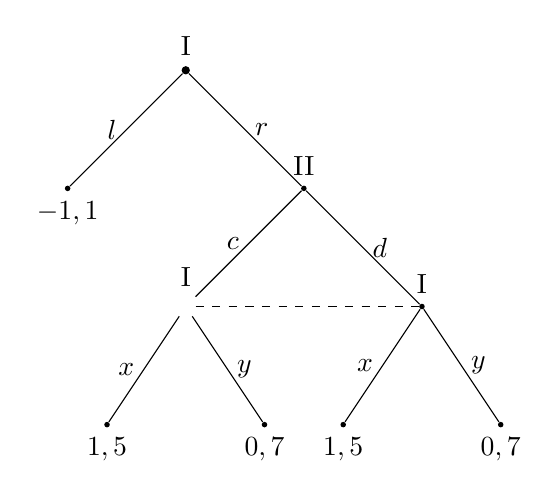
\begin{tikzpicture}[grow=down] % дерево
\tikzstyle{mystart} = [circle, minimum width=3pt,fill, inner sep=0pt] % starting node style
\tikzstyle{mydot} = [circle, minimum width=2pt,fill, inner sep=0pt] % decision node style
\tikzstyle{level 1}=[sibling distance=3cm] % расстояние между соседними узлами на одном уровне
\tikzstyle{level 2}=[sibling distance=3cm]
\tikzstyle{level 3}=[sibling distance=2cm]
\node[mystart, label=above: {I}] {} % создаем узел типа mydot, с пометкой "I" сверху и пустым текстом внутри узла
    child { node[mydot, label=below: {$-1,1$}] {}        
    edge from parent node[left] {$l$} }
    child { node[mydot, label=above: {II} ] {}        
        child { node[label=above: {I}] (a) {} 
                child { node[mydot, label=below: {$1,5$}] {}
               	edge from parent node[left] {$x$}}
                child { node[mydot, label=below: {$0,7$}] {}
               	edge from parent node[right] {$y$}  }
        edge from parent node[left] {$c$} }
        child { node[mydot, label=above: {I}] (b) {}
                child {	node[mydot, label=below: {$1,5$}] {}
              	edge from parent node[left] {$x$}}
                child { node[mydot, label=below: {$0,7$}] {}
               	edge from parent node[right] {$y$}  }
        edge from parent node[right] {$d$} }
    edge from parent node[right] {$r$} };
\draw[dashed] (a)--(b);
\end{tikzpicture}


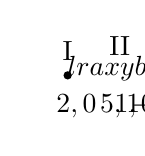
\begin{tikzpicture}
\tikzstyle{mydot} = [circle, minimum width=2pt,fill, inner sep=0pt] % decision node style
\tikzstyle{mystart} = [circle, minimum width=3pt, fill, inner sep=0pt] % starting node style
\tikzset{edge from parent/.style= {draw,  edge from parent path={(\tikzparentnode) -- (\tikzchildnode)}},
 every tree node/.style={mydot}} % make every tree node a decision node; we have to override the start node

\Tree 
    [.\node[mystart, label=above: I] {};  
        \edge node[above left] {$l$}; \node[ label=below: {$2,0$}] {}; 
        \edge node[above right] {$r$}; [.\node[ label=above right:II] {};  
            \edge node[left] {$a$}; [.\node (a) {};  
                \edge node[left] {$x$}; \node[ label=below: {$5,1$}] {}; 
                \edge node[right] {$y$}; \node[ label=below: {$1,0$}] {}; ] 
            \edge node[right] {$b$}; [.\node (b) {}; 
                \edge node[left] {$x$}; \node[ label=below: {$-1,4$}] {}; 
                \edge node[right] {$y$}; \node[ label=below: {$0,1$}] {}; ]   ]   ]
\draw[dashed] (a)--node[label=above:I] {}(b);
\end{tikzpicture}



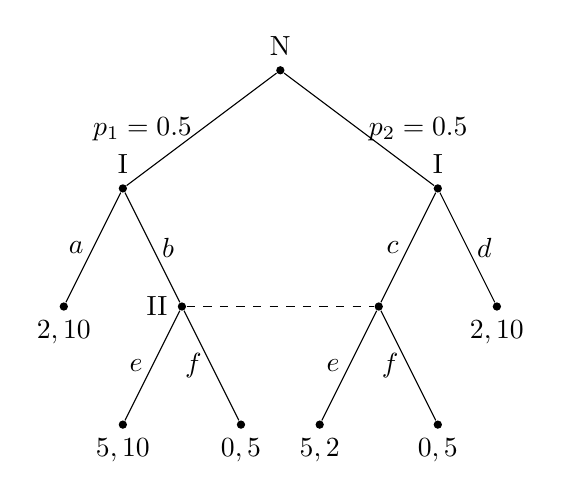
\begin{tikzpicture}[grow=down] % дерево
\tikzstyle{mydot} = [circle, minimum width=3pt,fill, inner sep=0pt] % размеры точки в центре узла
\tikzstyle{level 1}=[sibling distance=4cm] % расстояние между соседними узлами на одном уровне
\tikzstyle{level 2}=[sibling distance=1.5cm]
\tikzstyle{level 3}=[sibling distance=1.5cm]

\node[mydot, label=above: {N}] {}
	child { node[mydot, label=above: {I}] {}
			child { node[mydot, label=below: {$2,10$}] {}
     		edge from parent node[left] {$a$} }
			child { node[mydot, label=left: {II} ] (a) {}
					child { node[mydot, label=below: {$5,10$}] {}
					edge from parent node[left] {$e$} }
					child { node[mydot, label=below: {$0,5$}] {}
					edge from parent node[left] {$f$} }
	    	edge from parent node[right] {$b$} }
	edge from parent node[left] {$p_1=0.5$} }
	child { node[mydot, label=above: {I}] {}
			child { node[mydot] (b) {}
					child {	node[mydot, label=below: {$5,2$}] {}
					edge from parent node[left] {$e$} }
  					child {	node[mydot, label=below: {$0,5$}] {}
					edge from parent node[left] {$f$} }
			edge from parent node[left] {$c$} }
			child {	node[mydot, label=below: {$2,10$}] {}
			edge from parent node[right] {$d$} }
	edge from parent node[right] {$p_2=0.5$} } ;
\draw[dashed] (a)--(b);
\end{tikzpicture}

\begin{enumerate}
\item Укажите число стратегий каждого игрока 
\item Переведите игры в матричную форму
\end{enumerate}
Примечание: в играх с природой в матрицу пишут средний выигрыш 

\item Задана антагонистическая игра (в матрице указывается выигрыш для первого игрока):\\
$\begin{array}{c|ccc}
    {} &  d & e & f   \\
\hline
    a &  { - 2} & 1 & 3   \\
    b &  3 & x & { - 5}   \\
    c &  2 & { - 3} & 0   \\
\end{array}$\\
\begin{enumerate}
\item Допишите в матрицу выигрыши второго игрока;
\item Найдите осторожные стратегии обоих игроков при $x = 0$
\item Найдите осторожные стратегии обоих игроков при произвольном $x$
\end{enumerate}

\item Задана матрица игры:\\
$\begin{array}{c|ccc}
    {} &  {t_1 } & {t_2 } & {t_3 }   \\
\hline
    {l_1 } &  {\left( {0;0} \right)} & {\left( {0;0} \right)} & {\left( {0;0} \right)}   \\
    {l_2 } &  {\left( {0;0} \right)} & {\left( {1; - 3} \right)} & {\left( { - 3;1} \right)}   \\
    {l_3 } &  {\left( {0;0} \right)} & {\left( { - 3;1} \right)} & {\left( {1; - 3} \right)}   \\
\end{array}$
\begin{enumerate}
\item Существует ли последовательная игра с совершенной информацией (<<дерево без пунктиров>>) с такой матрицей? 
\item Существует ли последовательная игра с несовершенной информацией (<<дерево с пунктирами>>) с такой матрицей? 
\end{enumerate}

\item Deep Blue\\
Представим, что Вы играете партию в шахматы против компьютера. Сколько стратегий использует компьютер во время одной партии?

\item Есть несколько кучек камней. Два игрока ходят по очереди. За ход разрешается: либо взять любое положительное количество камней из одной кучки, либо поделить любую кучку на две новые непустые кучки. Проигрывает тот, кто не может сделать ход. Проигравший платит победителю 1 рубль. Игроки ходят по очереди.\\
Нарисуйте дерево игры, начинающейся с единственной кучки из 3 камней.

\item В кучке лежит 5 камней. Петя и Вася по очереди забирают камни из кучки. Петя ходит первым. За свой ход Петя может взять 1 или 3 камня, а Вася 2 или 3 камня. Проигрывает тот, кто не может сделать ход. Проигравший платит победителю рубль.
\begin{enumerate}
\item Нарисуйте дерево игры;
\item Переведите игру в матричную форму.
\item Найдите осторожные стратегии игроков.
\item Решите игру методом обратной индукции
\end{enumerate}

\item Задана антагонистическая игра в матричной форме. Определите, верно или не верно каждое утверждение:
\begin{enumerate}
\item При увеличении всех чисел матрицы на единицу осторожные стратегии игроков не изменятся.
\item При умножении всех чисел на минус единицу осторожные стратегии игроков не изменятся.
\item При транспонировании матрицы осторожные стратегии игроков поменяются местами (т.е. осторожные стратегии второго игрока станут осторожными стратегиями первого игрока и наоборот).
\end{enumerate}

\item С чего все начиналось... \\
Париж, Людовик XIV, 1654 год, высшее общество говорит о рождении новой науки - теории вероятностей. Ах, кавалер де Мере, <<fort honn\^ete homme sans \^etre math\'ematicien>> <<благородный человек, хотя и не математик>>... Старая задача, неправильные решения которой предлагались тысячелетиями (например, одно из неправильных решений предлагал изобретатель двойной записи, кумир бухгалтеров, Лука Пачоли) наконец решена правильно!\\
Два игрока одинаковой силы играют в некую игру до шести побед. Игрок первым выигравший шесть партий (не обязательно подряд) получает 800 луидоров. К текущему моменту первый игрок выиграл 5 партий, а второй - 3 партии. Они вынуждены прервать игру в данной ситуации.\\
Как им поделить приз по справедливости?

\item Кортес\\
Кортес с бандой головорезов высадился на берегу. Кортес выбирает, нападать ли на деревушку или нет. Местная деревушка может либо сразу перейти в подчинение Кортеса, либо принять бой. Если деревушка примет бой, то выбор появится у Кортеса: либо драться до победного конца, либо после первых потерь бежать на кораблях обратно. Ценность деревушки для Кортеса – одна единица, ценность собственных головорезов – 2 единицы. Если Кортес будет драться до конца, то деревушка будет взята, но большинство головорезов погибнет в бою. Для жителей деревушки – главное остаться в живых, сохранить при этом независимость, конечно, желательно. 
\begin{enumerate}
\item Нарисуйте дерево игры и найдите обратно-индукционный исход.
\item Нарисуйте дерево игры и найдите обратно-индукционный исход в случае, если Кортес ограничил свои возможности --- сжег корабли.
\end{enumerate}

\end{enumerate}


\section{Доминирование, NE в смешанных (технический семинар) }

$[$Slantchev$]$ - глава Dominance, Nash Equilibrium, Symmetry; $[$IGT$]$ - глава 2,3,4, 11\\


\textbf{Равновесие Нэша}. Nash equilibrium. NE.\\
-- Профиль стратегий, в котором ни один игрок не захочет сменить свою стратегию, даже если узнает стратегии других игроков. 

\textbf{Парето оптимум}. Pareto optimum. PO.\\
-- Вектор платежей называется Парето-оптимальным, если любой другой вектор платежей хуже хотя бы для одного игрока.

\textbf{Статическая игра, Нормальная форма записи} \\
Формальное описание статической игры содержит: список игроков; для каждого игрока: список стратегий, зависимость выигрыша от выбранных всеми игроками стратегий. 

\textbf{Доминирование стратегий} \\
Стратегия <<a>> строго доминирует стратегию <<b>>, если вне зависимости от действий других игроков <<a>> приносит больший выигрыш, чем <<b>>.

\textbf{Смешанная стратегия} \\
Смешанная стратегия --- случайный эксперимент, в результате которого выбирается одна из чистых стратегий.


%Исход, в котором платеж ни одного игрока нельзя улучшить, не ухудшив при этом платеж хотя бы одного другого игрока.\\

Разные замечания: 
\begin{itemize}
\item Смешивать стратегии $a$ и $b$ оптимально тогда и только тогда, когда $a$ и $b$ приносят одинаковый платеж, а остальные стратегии - не больший. \\
\item Если предложить игрокам перейти из Парето оптимального исхода в любой другой, то хотя бы один игрок не согласится.\\
\item Развернутая форма -- дерево игры
\end{itemize}

\begin{enumerate}

\item Рассмотрим игру $\begin{array}{c|ccc}
    {} &  {t_1 } & {t_2 } & {t_3 }   \\
\hline
    {l_1 } &  {\left( {2;8} \right)} & {\left( {1;6} \right)} & {\left( {9;20} \right)}   \\
    {l_2 } &  {\left( {7;7} \right)} & {\left( {6;8} \right)} & {\left( {2;6} \right)}   \\
\end{array}$
\begin{enumerate}
\item Какая стратегия является наилучшим ответом второго игрока на стратегию $l_2 $?
\item Дополните матрицу смешанной стратегий первого игрока $\frac{1}{3}l_1  + \frac{2}{3}l_2 $
\item Какая стратегия является наилучшим ответом второго игрока на стратегию $\frac{1}{3}l_1  + \frac{2}{3}l_2 $?
\item Найдите все смешанные стратегии (смешиваются $t_2 $  и $t_3 $), которые строго доминируют чистую стратегию $t_1 $ в исходной матрице. 
\end{enumerate}

\item Найдите равновесия Нэша в смешанных стратегиях: \\
а) $\begin{array}{c|ccc}
& t_{1} & t_{2} & t_{3} \\
\hline
s_{1} & (2;4) & (3;4) & (0;0) \\
s_{2} & (1;2) & (4;7) & (1;8) \\
\end{array}$;
б) $\begin{array}{c|ccc}
& t_{1} & t_{2} & t_{3} \\
\hline
s_{1} & (3;3) & (1;1) & (5;3) \\
s_{2} & (1;2) & (2;2) & (1;1) \\
\end{array}$;
в) $\begin{array}{c|cc}
& t_{1} & t_{2} \\
\hline
s_{1} & 5 & 1 \\
s_{2} & 2 & 3 \\
s_{3} & 1 & 6 \\
\end{array}$ 

\item Два игрока играют в статическую игру. Первый выбирает $x\in [0;3]$, второй одновременно выбирает $y\in [0;4]$. Платежные функции имеют вид $U_{1}(x,y)=-x^{2}+2xy+6y+cos(y)$, $U_{2}(x,y)=-y^{2}-8xy+6y+arctg(x)$. 
\begin{enumerate}
\item Изобразите функции наилучших ответов в осях $(x,y)$ 
\item Найдите равновесие Нэша в чистых стратегиях 
\end{enumerate}

\item $\begin{array}{c|ccc}
& d & e & f \\
\hline
a & (3;5) & (1;0) & (2;2)\\
b & (-1;0) & (4;4) & (7;2)\\
c & (1;7) & (2;3) & (4;7)\\
\end{array}$ 
\begin{enumerate}
\item Придумайте смешанную стратегию, строго доминирующую стратегию $c$ 
\item Последовательно вычеркивая строго доминируемые стратегии сведите матрицу к размеру $(2\times 2)$ 
\item Найдите все равновесия Нэша в смешанных стратегиях 
\end{enumerate}

\item Два тигра \\
Два тигра заметили двух антилоп. Маленькую, весом в один условный килограмм, и большую, весом в $a > 1$ условных килограммов. Они одновременно принимают решение, за какой антилопой погнаться. Тигры всегда догоняют антилоп. \textit{Тигр: Если хотят, то конечно.} Если тигры выберут одну антилопу, то они поделят ее поровну. 
\begin{enumerate}
\item Запишите игру в матричной форме;
\item Найдите все равновесия Нэша в чистых и смешанных стратегиях в зависимости от $a$
\end{enumerate}

\item Для игр: \\
$\begin{array}{c|ccc}
    {} &  d & e & f   \\
\hline
    a &  (3;2) & (1;1) & (7;1)   \\
    b &  (0;1) & (3;3) & (-3;2)   \\
    c &  (1;4) & (2;2) & (0;0)   \\
\end{array}$;
 $\begin{array}{c|ccc}
    {} &  d & e & f   \\
\hline
    a &  (0;2) & (2;1) & (-2;1)   \\
    b &  (0;1) & (3;3) & (-3;4)   \\
    c &  (1;0) & (2;2) & (0;0)   \\
\end{array}$;
 $\begin{array}{c|ccc}
    {} &  d & e & f   \\
\hline
    a &  (2;2) & (3;2) & (7;1)   \\
    b &  (0;1) & (3;3) & (-3;1)   \\
    c &  (0;4) & (-1;2) & (0;0)   \\
\end{array}$;\\
\begin{enumerate}
\item Вычеркнув строго доминируемые стратегии сведите данные игры к размеру $(2\times 2)$ При вычеркивании можно использовать смешанные стратегии! 
\item Найдите равновесия Нэша в смешанных стратегиях;
\item Найдите Парето-оптимальные точки в чистых стратегиях 
\end{enumerate}

\item Придумайте биматричную игру размером $\left( {3 \times 3} \right)$, в которой с помощью вычеркивания нестрого доминируемых стратегий можно оставить ровно один исход, причем результат зависит от порядка вычеркивания.

\item Два игрока одновременно называют натуральное число от 1 до 5. Первый игрок получает выигрыш, равный квадрату разности чисел. Второй игрок получает выигрыш равный наименьшему числу. \\
Найдите равновесия Нэша в чистых стратегиях и Парето-оптимальные точки.

\item Студенты и волшебная шкатулочка \\
Вася и Петя нашли волшебную шкатулочку. Если в нее положить деньги и сказать <<Ахалай Махалай>>, то сумма, лежащая в шкатулке увеличивается в полтора раза. Один недостаток: работает только раз! Петя и Вася решили поступить так: каждый положит в шкатулку сколько хочет, потом они скажут <<Ахалай Махалай>> и поделят всю сумму поровну.
\begin{enumerate}
\item Что является стратегией игрока?
\item Представьте эту игру в \textit{нормальной форме}
\item Можно ли представить игру в матричной форме? Почему?
\item Найдите равновесие Нэша;
\end{enumerate}

\item Делим пирог\\
Мама одновременно спрашивает двух братьев, какую долю пирога каждый хотел бы получить. Братья получают то, что попросили, если пирога хватает (остаток при этом мама уносит на работу). Если братья вместе запросили больше, чем целый пирог, то они не получают ничего.
\begin{enumerate}
\item Представьте игру в нормальной форме;
\item Найдите все равновесия Нэша в чистых стратегиях
\end{enumerate}

\item Три игрока одновременно называют одно из чисел: ноль или один. Если все трое называют единицу, то их выигрыш равен 10, если все трое называют ноль, то их выигрыш равен 5.
\begin{enumerate}
\item Найдите Парето-оптимальные точки в чистых стратегиях;
\item Найдите равновесия Нэша в чистых стратегиях 
\item Найдите равновесия Нэша в смешанных стратегиях 
\end{enumerate}

\item Экология \\
Три фирмы, использующие воду из одного озера, одновременно решают, очищать ли им сточные воды, сбрасываемые в то же озеро. Очистка воды означает издержки равные единице. Если воду не очищают две или три фирмы, то каждая из трех фирм несет дополнительные издержки в размере трех единиц.
\begin{enumerate}
\item Найдите все равновесия Нэша в чистых стратегиях
\item Найдите все равновесия Нэша в смешанных стратегиях
\end{enumerate}

\item Рассмотрим игру $\begin{array}{c|ccc}
    {} &  {t_1 } & {t_2 } & {t_3 }   \\
\hline
    {l_1 } &  {\left( {2;x} \right)} & {\left( {1;4} \right)} & {\left( {9;20} \right)}   \\
    {l_2 } &  {\left( {7;y} \right)} & {\left( {6;8} \right)} & {\left( {2;4} \right)}   \\
\end{array}$
\begin{enumerate}
\item Пусть $y = 5$. При каких $x$  существует смешанная стратегия, строго доминирующая чистую стратегию $t_1 $? 
\item Изобразите на плоскости множество таких пар $\left( {x,y} \right)$, при которых существует чистая стратегия, строго доминирующая стратегию $t_1 $. 
\item Изобразите на плоскости множество таких пар $\left( {x,y} \right)$, при которых существует смешанная стратегия, строго доминирующая стратегию $t_1 $ 
\end{enumerate}

\item Вопросы о разном... 
\begin{enumerate}
\item Может ли в равновесие Нэша входить строго доминируемая стратегия? 
\item Может ли в равновесие Нэша входить нестрого доминируемая стратегия? 
\item Могут ли все исходы игры быть равновесными Нэша? 
\item Может ли в игре не быть ни одного равновесия Нэша в чистых стратегиях? 
\item Может ли в игре не быть ни одного равновесия Нэша в смешанных стратегиях? 
\item Может ли существовать стратегия, на которую не существует оптимального ответа? 
\item Может ли игра в развернутой форме быть антагонистической?
\item Сколько смешанных стратегий у первого игрока, если у первого игрока две чистых стратегии, а у второго – три чистых стратегии?
\end{enumerate}

\end{enumerate}
\section{Практикум по NE}

\begin{enumerate}
\item Дуополия Бертрана \\
Две фирмы назначают цены на свою продукцию. Предельные издержки обеих фирм равны нулю. Рыночный спрос описывается функцией $Q = \max \left\{ {1 - P,0} \right\}$. Весь спрос достается фирме, назначившей наименьшую цену; если фирмы назначили одинаковую цену, то спрос делится между ними поровну.
\begin{enumerate}
\item Изобразите на плоскости стратегии равновесные Нэша и Парето оптимальные точки;
\item Грандиозное предложение! Фирмы снова одновременно назначают цены, но каждая фирма обязуется вернуть покупателю разницу в цене товара, если конкурент продает дешевле. Как изменятся множества равновесных Нэша стратегий и Парето оптимальных точек?
\end{enumerate}

\item Старику на остановке плохо. Рядом находятся еще $n$  человек. Каждый из них, независимо от других, может либо вызвать скорую с помощью мобильного, либо ничего не делать. Если никто не вызовет скорую, то старик умрет. Если скорая будет вызвана, то старик будет спасен. Если старик умрет, то полезность каждого равна 0, если старик остается в живых, то полезность каждого равна 1. Издержки телефонного звонка равны 0.001.
\begin{enumerate}
\item Найдите все равновесия Нэша в чистых стратегиях;
\item Найдите симметричное равновесие Нэша в смешанных стратегиях;
\item Как зависит от  $n$  вероятность получения помощи?
\end{enumerate}

\item Выкуп доли\\
Доля Маши в ЗАО <<Красивое платье>> составляет  $s$, а доля Кати -  $\left(1-s\right)$. Маша и Катя решили отказаться от дальнейшего сотрудничества. У ЗАО должна быть одна владелица! 
Ценность ЗАО для каждой владелицы - случайная величина  $\nu _{i} $  равномерно распределенная на  $\left[0;1\right]$.
\begin{enumerate}
\item Маша и Катя решили попробовать аукцион. Оба игрока одновременно называют цену ЗАО. Тот, кто назвал более высокую цену, должен выкупить акции партнера по предложенной им самим цене (более высокой). Найдите равновесие Нэша в линейных стратегиях, т.е. предлагаемая каждым игроком цена должна иметь вид  $b_{i} =\beta \nu _{i} $ , где  $v_{i} $  - его оценка стоимости ЗАО, а    $\beta $  - константа. Не забудьте случай  $s=0$ , т.е. Маша продавец, а Катя - покупатель. Возможно ли, что акции достанутся тому, кто их меньше ценит?
\item Решите вариант задачи: тот, кто назвал более высокую цену, должен выкупить акции партнера по предложенной партнером более низкой цене. 
\end{enumerate}

\item Что предложил Warren Buffet? \\
Парламент поделен на две партии: республиканцы и демократы. Для принятия реформы необходима ее поддержка обеими партиями. Реформа безразлична обеим партиям. Warren Buffet предложил, чтобы какой-нибудь миллиардер выступил со следующим обещанием: Если реформа не будет принята, то партия, поддержавшая реформу во время голосования получит 1 000 000 000\$ (Один миллиард долларов). Партии голосуют одновременно  за или против реформы. Каждая партия хотела бы получить деньги и не хотела бы, чтобы деньги достались конкурентам. Допустим, что нашелся миллиардер, выступивший с таким заявлением, а партии поверили заявлению миллиардера.
\begin{enumerate}
\item Представьте игру в нормальной (матричной) форме; 
\item Найдите равновесие Нэша
\item Чего добился миллиардер? 
\end{enumerate}
Тигр: сам Buffet с подобным заявлением не выступил!\\
Source: Game theory at work 

\item Конверты \\
В пяти конвертах спрятаны суммы в 10\$, 20\$, 40\$, 80\$ и 160\$. Случайным образом выбираются два конверта с соседними суммами и выдаются игрокам. {\it Тигр: А в конвертах - это взятки?} Каждый игрок открывает свой конверт и выбирает, хочет ли он оставить себе сумму или хочет обменяться. Обмен происходит, если оба игрока согласны обменяться.
\begin{enumerate}
\item  Сколько чистых стратегий у каждого игрока?
\item Найдите все равновесия Нэша в чистых и смешанных стратегиях.
\end{enumerate}
Source: exam Jannssen 

\item На аукционе продаются 12 стульев работы мастера Гамбса (одним лотом). Ценность стульев для каждого из $n$ покупателей - случайная величина, равномерная на $[0;1]$. Покупатели одновременно назначают цены. Победитель аукциона - тот, кто назвал самую высокую цену. Стулья достаются победителю. Победитель платит названную им цену. 
\begin{enumerate}
\item Найдите симметричное равновесие Нэша в чистых стратегиях. Найдите ожидаемую выручку устроителей аукциона. 
\item Изменим правила: победитель платит названную им цену плюс комиссионный сбор в 10\%. Найдите равновесие Нэша и ожидаемую выручку устроителей. 
\item Изменим правила: победитель платит названную им цену плюс комиссионный сбор равный $0.05$. Найдите равновесие Нэша и ожидаемую выручку устроителей. 
\item Изменим правила: победитель платит вторую по величине цену. Например, если игроки назвали цены 100, 200, 300 и 400, то победитель - тот, кто сказал 400, но платит он 300. Найдите равновесие Нэша и ожидаемую выручку устроителей. 
\end{enumerate}

\item Морской бой в узком проливе \\
Первый игрок располагает корабль размером $1\times 2$ на поле размером $1\times 4$. Второй игрок не зная выбор первого делает выстрел в одну из четырех клеток поля. Задача первого - спасти корабль, задача второго - потопить. 
\begin{enumerate}
\item Постройте матрицу игры 
\item Найдите все равновесия Нэша в смешанных стратегиях 
\end{enumerate}

\item (*) Мусоросжигательный завод \\
В стране  $n$  городов. Около одного из них нужно построить большой мусоросжигательный завод. Предположим, что ущерб от мусоросжигательного завода для жителей каждого города - случайная величина, равномерно распределенная на отрезке  $\left[0;1\right]$ . Каждый город объявляет компенсацию, требуемую за постройку мусоросжигательного завода поблизости. Завод строят около города, запросившего наименьшую компенсацию. Деньги выплачивают остальные города в равной пропорции.\\
Найдите симметричное равновесие Нэша в чистых стратегиях;

\item Мост \\
Из пункта $A$ в пункт $D$ можно попасть двумя путями - через B или
через C. Если по дороге AB едет $x$ машин, то время в пути каждой
из них будет равно $f_{AB}(x)=x+32$. Для других отрезков пути
функции равны: $f_{BD}(x)=5x+1$, $f_{CD}(x)=x+32$ и
$f_{AC}(x)=5x+1$.
Каждое утро из города $A$ в город $D$ едет 6 машин. \\
\begin{figure}[h]
    \includegraphics{game.5}
\end{figure} 
\begin{enumerate}
\item Сколько машин и по какой дороге едет в равновесии Нэша?
Сколько им требуется времени, чтобы добраться из $A$ в $D$? 
\item Как изменятся ответы, если между городами $B$ и $C$ построен
удобный мост, такой что $f_{BC}=0$? 
\end{enumerate}

\item Два человека пришли в кабак. У одного из них 10 золотых, у второго~--- 6 золотых. Каждый может тратить деньги на выпивку или на музыку.
Музыка является общественным благом --- ее слышат все. Выпивка -
частным. Полезности равны $u_{1}=(m_{1}+m_{2})d_{1}$ и
$u_{2}=(m_{1}+m_{2})d_{2}$, где $m_{i}$ и $d_{i}$ - расходы $i$-го
человека на музыку и выпивку. Предположим, что деньги бесконечно
делимы. 
\begin{enumerate}
\item Найдите равновесие Нэша 
\item Что изменится в случае, если у второго 2 золотых? 
\end{enumerate}

\item Президент \\
Два гражданина борются за пост президента страны. Каждый из них выбирает свою политическую позицию. Под позицией мы будем понимать натуральное число от 1 до 99, где число один означает крайне левую позицию, а 99 – крайне правую. Если оба гражданина занимают одну политическую позицию, то голоса делятся поровну. Если позиции различны, то каждый житель (в стране 99 жителей) выбирает того кандидата, к которому он ближе расположен. Если жителю все равно, то его голос делится поровну между кандидатами.
\begin{enumerate}
\item Найдите все исходы, которые остаются в результате последовательного вычеркивания нестрого доминируемых стратегий
\item Найдите равновесие Нэша
\end{enumerate}

\item Всеобщность знания\\
$\begin{array}{c|cc}
    {} &  s & c   \\
\hline
    s &  {\left( {1;1} \right)} & {\left( { - 2; - 1} \right)}   \\
    c &  {\left( { - 1; - 2} \right)} & {\left( { - 1; - 1} \right)}   \\
\end{array}$\\
В уездном городе $N$ живут игроки двух типов: <<безумцы>> и рациональные. При встрече в городе $N$ принято играть в игру, изображенную слева. Рациональные игроки играют стратегию, приносящую наибольший выигрыш, а безумцы – стратегию $c$.\\
Как-то случилось Петя попасть в этот город и встретится с одним рациональным аборигеном. Они никогда раньше не виделись и никогда больше не увидятся. Петя знает, что абориген - рационален. Абориген знает, что Петя - рационален. Петя ошибочно полагает, что абориген считает его безумцем. Абориген знает о Петиной ошибке.\\
Найдите все равновесия Нэша в этой матрице. Какое из них будет сыграно?

\item О пользе гадалок замолвите слово... \\
Маша пишет на бумажках два любых различных натуральных числа по своему выбору. Одну бумажку она прячет в левую руку, а другую - в правую. Саша выбирает любую Машину руку. Маша показывает число, написанное на выбранной бумажке. Саша высказывает свою догадку о том, открыл ли он большее из двух чисел или меньшее. Если Саша не угадал, то Маша выиграла.\\
Приведите пример Сашиной смешанной стратегии, гарантирующей ему вероятность выигрыша строго более 50\% вне зависимости от стратегии Маши (!) \\
Подсказка: представьте себе, что перед выбором руки и высказыванием догадки Саша может обратиться к потомственной гадалке в пятом поколении Глафире Лукитичне Пуассоновой (500\% гарантия, снятие порчи и сглаза без греха и ущерба для здоровья, исправляет некачественную работу шарлатанов). Глафира Лукитична (ничего не зная о Маше!) называет наугад число $X=N+0.5$, где $N$ - Пуассоновская случайная величина с $\lambda=1$.  \\
Source: Winkler, games people don't play 

\item Две фирмы производят одинаковый продукт. Они одновременно выбирают свои объемы выпуска, $q_1$ и $q_2$. Предельные издержки выпуска равны соответственно $1$, $2$. Каждая фирма максимизирует свою прибыль. Обратная функция спроса имеет вид $p=10-q$. Найдите равновесие Нэша.

\end{enumerate}

\section{SPNE (Subgame Perfect Nash Equilibrium), обратная индукция продолжение}

$[$IGT$]$ - главы 5,6,7; $[$Slantchev$]$ - глава Perfect Equilibria in Extensive Form Games (кроме части 2) \\

Подыгра --- часть игры, начинающаяся с определенного узла (конкретный узел и все узлы <<ниже>> него). При <<отрезании>> подыгры от всей игры не должны <<разрываться>> информационные множества\\
Равновесие Нэша, совершенное в подыграх (SPNE) --- профиль стратегий, оказывающийся равновесием Нэша в каждой подыгре включая всю игру. В играх с совершенной информацией совпадает с методом обратной индукции. \\


\begin{enumerate}
\item 1.1. 1.2. 1.3. \\

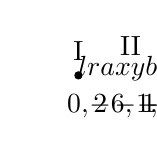
\begin{tikzpicture}
\tikzstyle{mydot} = [circle, minimum width=2pt,fill, inner sep=0pt] % decision node style
\tikzstyle{mystart} = [circle, minimum width=3pt, fill, inner sep=0pt] % starting node style
\tikzset{edge from parent/.style= {draw,  edge from parent path={(\tikzparentnode) -- (\tikzchildnode)}},
 every tree node/.style={mydot}} % make every tree node a decision node; we have to override the start node

\Tree 
    [.\node[mystart, label=above: I] {};  
        \edge node[above left] {$l$}; \node[ label=below: {$0,2$}] {}; 
        \edge node[above right] {$r$}; [.\node[ label=above right:II] {};  
            \edge node[left] {$a$}; [.\node (a) {};  
                \edge node[left] {$x$}; \node[ label=below: {$-6,-6$}] {}; 
                \edge node[right] {$y$}; \node[ label=below: {$-1,1$}] {}; ] 
            \edge node[right] {$b$}; [.\node (b) {}; 
                \edge node[left] {$x$}; \node[ label=below: {$1,-1$}] {}; 
                \edge node[right] {$y$}; \node[ label=below: {$-3,-3$}] {}; ]   ]   ]
\draw[dashed] (a)--node[label=above:I] {}(b);
\end{tikzpicture}

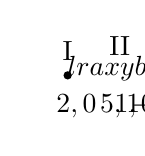
\begin{tikzpicture}
\tikzstyle{mydot} = [circle, minimum width=2pt,fill, inner sep=0pt] % decision node style
\tikzstyle{mystart} = [circle, minimum width=3pt, fill, inner sep=0pt] % starting node style
\tikzset{edge from parent/.style= {draw,  edge from parent path={(\tikzparentnode) -- (\tikzchildnode)}},
 every tree node/.style={mydot}} % make every tree node a decision node; we have to override the start node

\Tree 
    [.\node[mystart, label=above: I] {};  
        \edge node[above left] {$l$}; \node[ label=below: {$2,0$}] {}; 
        \edge node[above right] {$r$}; [.\node[ label=above right:II] {};  
            \edge node[left] {$a$}; [.\node (a) {};  
                \edge node[left] {$x$}; \node[ label=below: {$5,1$}] {}; 
                \edge node[right] {$y$}; \node[ label=below: {$1,0$}] {}; ] 
            \edge node[right] {$b$}; [.\node (b) {}; 
                \edge node[left] {$x$}; \node[ label=below: {$-1,4$}] {}; 
                \edge node[right] {$y$}; \node[ label=below: {$0,1$}] {}; ]   ]   ]
\draw[dashed] (a)--node[label=above:I] {}(b);
\end{tikzpicture}

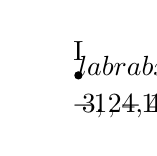
\begin{tikzpicture}
\tikzstyle{mydot} = [circle, minimum width=2pt,fill, inner sep=0pt] % decision node style
\tikzstyle{mystart} = [circle, minimum width=3pt, fill, inner sep=0pt] % starting node style
\tikzset{edge from parent/.style= {draw,  edge from parent path={(\tikzparentnode) -- (\tikzchildnode)}},
 every tree node/.style={mydot}} % make every tree node a decision node; we have to override the start node

\Tree 
    [.\node[mystart, label=above: I] {};  
        \edge node[above left] {$l$}; [.\node (a) {}; 
            \edge node[left] {$a$}; \node[ label=below: {$3,2$}] {}; 
            \edge node[right] {$b$}; \node[ label=below: {$-1,-1$}] {}; ] 
        \edge node[above right] {$r$}; [.\node (b) {};  
            \edge node[left] {$a$}; \node[ label=below: {$4,4$}] {};  
            \edge node[right] {$b$}; [.\node[ label=above right: I] {}; 
                \edge node[left] {$x$}; \node[ label=below: {$1,5$}] {}; 
                \edge node[right] {$y$}; \node[ label=below: {$0,7$}] {}; ]   ]   ]
\draw[dashed] (a)--node[label=above:II] {}(b);
\end{tikzpicture}


\begin{enumerate}
\item Посчитайте число подыгр;
\item Найдите равновесия Нэша, совершенные в подыграх 
\end{enumerate}

\item Первый игрок называет неотрицательное число $x$. Затем второй игрок, зная число первого, называет неотрицательное число $y$. Выигрыши игроков определяются по формулам: $u^I \left( {x,y} \right) =  - x^2  + 4xy - y^2  + 11$ и $u^{II} \left( {x,y} \right) =  - 2y^2  + xy - 4x^2  + 12 + x + 2y$.
\begin{enumerate}
\item Что представляют собой стратегии игроков?
\item Найдите равновесие Нэша, совершенное в подыграх (примените метод обратной индукции)
\item Приведите пример равновесия Нэша, не совершенного в подыграх
\item Как изменится ответ, если второй игрок выбирает $y$ одновременно с первым?
\item Найдите равновесие Нэша, совершенное в подыграх, для случая $u^{II} \left( {x,y} \right) =  - y^2  + 6xy - 4x^2  + 12 + x - 2y$
\item Найдите равновесие Нэша, совершенное в подыграх, для случая $u^{II} \left( {x,y} \right) =  - y^2  + 8xy - 4x^2  + 12 + x + 2y$
\end{enumerate}

\item Четыреста лет назад\par
В 1612 г. в Лионе появилась книга поэта и математика Баше де Мезирьяка (Claude Gaspar Bachet de M\'eziriac\footnote{Баше де Мезирьяк перевел с греческого на латынь Арифметику Диофаната, на полях которой Ферма сформулировал свою великую теорему}) <<Занимательные и приятные числовые задачи>> (Probl\`emes plaisants et d\'electables qui se font par les nombres). В ней была предложена следующая игра. Двое по очереди называют числа от 1 до 10, выигрывает тот, кто первым доведет сумму до 100. В чью пользу эта игра?\par
Ссылка на переиздание 1884 года \url{http://cnum.cnam.fr/DET/8PY45.html}, задача 22. 

\item 
В кучке 121 камень. Петя и Вася ходят по очереди, начинает Петя. Петя за один ход может взять 1 или 3 камня, а Вася -- 1 или 4 камня. Проигрывает тот, кто не может сделать ход по правилам (выигрывает взявший последний камень). Кто выигрывает Петя или Вася? Если выигрывает Петя, то с какого хода ему следует начать?

\item <<Набери чет>>\\
В кучке 135 камней, двое игроков по очереди забирают себе от 1 до 4 камней. Выигрывает тот, кто к концу игры наберет четное число камней. В чью пользу эта игра? Если в пользу первого, то с какого хода следует начать игру?\\
Подсказка: обратная индукция на «двух линиях», как в предыдущей задаче.

\item 
Первоначально фишка расположена в узле А. Двое игроков по очереди могут двигать фишку на один ход в любом направлении, которое указано стрелочкой. Тот, кто не сможет сделать очередной ход, проиграл. В чью пользу эта игра? Если в пользу первого, то с какого хода следует начать игру?\\
\begin{figure}[!htbp]
    \includegraphics{game.27} 
\end{figure}

\item <<Одинокий ферзь>>\\
Шахматная доска, одинокий раненый ферзь стоит на h6. Раненый ферзь как и ферзь может двигаться на любое число клеток, но только влево или вниз, или влево-вниз. Двое игроков ходят по очереди, тот кто переставит ферзя на а1 выиграл. В чью пользу эта игра? Если в пользу первого, то с какого хода следует начать игру?\\
Подсказка: попробуйте обратную индукцию на шахматной доске\\
\def\mylist{Qh6}
\setchessboard{setpieces=\mylist,showmover=false}
\chessboard

\item 
В первой кучке – 6 камней, во второй – 7 камней. Вася и Петя ходят по очереди. Петя ходит первым.  Игрок делающий ход может выбрать одну из кучек и из нее взять один, два или три камня.
\begin{enumerate}
\item Кто выигрывает, Вася или Петя, если цель игры – взять самый последний камень?
\item Кто выигрывает, Вася или Петя, если проигрывает тот, кто взял самый последний камень?
\end{enumerate}
Подсказка: обратная индукция на плоскости.

\item 
Определите, истинно или ложно каждое утверждение:
\begin{enumerate}
\item Равновесие, совершенное в подыграх, всегда является равновесием Нэша
\item Обратно-индукционный исход всегда является равновесием, совершенным в подыграх
\item В конечной последовательной игре с полной совершенной информацией обязательно существует равновесие, совершенное подыграх
\item Если перевести последовательную игру в матричную форму и вычеркнуть нестрого доминируемую стратегию, то можно потерять равновесие, совершенное в подыграх
\end{enumerate}

\item 
Игра трех игроков представлена на рисунке 
\begin{enumerate}
\item Найдите все равновесия Нэша в чистых стратегиях; Подсказка: нарисуйте две матрицы; первый игрок выбирает матрицу, второй – строку, третий – столбец
\item Найдите все равновесия в чистых стратегиях, совершенные в подыграх;
\end{enumerate}
\begin{figure}[!htbp]
    \includegraphics{game.21}
\end{figure}

\item Судья и потерпевший\\
Ущерб – случайная величина $v$, равновероятно принимающая любое значение из $\left\{ {0;1;...;99} \right\}$. Потерпевший точно знает величину ущерба $v$, а судья знает лишь распределение. Потерпевший выбирает один из двух вариантов: честно задекларировать величину ущерба или не говорить ничего. Судья выбирает величину компенсации $R$.\\
Полезность потерпевшего $U_1  = R - v$. Полезность судьи $U_2  =  - \left( {v - R} \right)^2$.\\
Найдите равновесия Нэша, совершенные в подыграх.

\item Развод \\
Джон и Бэтти нужно поделить виллу, яхту, акции (Тигр: Контрольный пакет акций свечного заводика в Самаре) и автомобиль. Они условились на следующей процедуре дележа: каждый забирает себе один предмет по очереди.\\
Предпочтения выглядят так (в порядке убывания ценности):\\
Бэтти: яхта, вилла, акции, автомобиль. Джон: вилла, акции, автомобиль, яхта\\
Найдите равновесие, совершенное в подыграх, если очередность выбор предметов Бэтти-Джон-Бэтти-Джон;

\item Джон и Бэтти помирились \\
Во время дележа имущества Джон и Бэтти помирились, и решили культурно отдохнуть. Предпочтения (снова в порядке убывания ценности).\\
Бэтти: балет, казино, бассейн, бокс. Джон: бокс, бассейн, казино, балет.\\
Они по очереди вычеркивают нежелательную альтернативу, до тех пор, пока не останется только одна. Найдите равновесия Нэша, совершенные в подыграх, для варианта очередности Бэтти-Джон-Бэтти-Джон\\
Source: Брамс 

\item 
Неправильная монетка выпадает <<орлом>> с вероятностью $0<p<1$. Первый игрок знает результат выпадения монетки, второй – нет. Первый игрок объявляет второму, как выпала монетка (при этом он может соврать). Затем второй делает свою догадку о том, как в действительности выпала монетка. За свою правдивость первый игрок получает единицу полезности и еще две единицы получает в том случае, если второй скажет «орел». Второй игрок получает единицу полезности, если верно угадает, как выпала монетка. Найдите все равновесия Нэша, совершенные в подыграх.

\item Две сверхдержавы\\
Две сверхдержавы играют в одновременную игру и выбирают, нажимать ли красную кнопку запуска стратегических ядерных ракет, или нет. Эффективных систем защиты от ядерного удара нет. Матрица игры имеет вид:\\
$\begin{array}{c|cc}
    {} &  {press} & {not}   \\
\hline
    {press} &  {\left( { - a; - a} \right)} & {\left( {1; - a} \right)}   \\
    {not} &  {\left( { - a;1} \right)} & {\left( {0;0} \right)}   \\
\end{array}$
\begin{enumerate}
\item Найдите все равновесия Нэша в этой игре;
\item Допустим, обе сверхдержавы создали системы раннего обнаружения запуска ядерных ракет. Если одна из сверхдержав не запустила ракеты, а другая – запустила, у незапустившей появляется возможность изменить свою решение. Для простоты будем считать, что если ни одна из держав не нажала красную кнопку, то игра сразу оканчивается. Отменить запуск по-прежнему нельзя. 
\item Изобразите дерево игры
\item Найдите равновесия Нэша совершенные в подыграх в измененной игре; 
\end{enumerate}
Тигр: они доиграются... 

\item  Три фирмы производят одинаковый продукт. Сначала первая фирма выбирает свой объем выпуска, $q_1$. Затем вторая и третья фирмы, зная $q_1$, выбирают одновременно свои объемы выпуска, $q_2$ и $q_3$. Предельные издержки выпуска равны соответственно $1$, $2$ и $4$. Обратная функция спроса имеет вид $p=10-q$, где $q$ --- суммарный выпуск трех фирм, $q=q_1+q_2+q_3$. Каждая фирма максимизирует свою прибыль.
\begin{enumerate}
\item Найдите равновесие Нэша, совершенное в подыграх
\item Какие объемы выпуска будут выбирать фирмы в найденном равновесии?
\end{enumerate}

\item  Три фирмы производят одинаковый продукт. Сначала первая и вторая фирмы выбирают одновременно свои объемы выпуска, $q_1$ и $q_2$. Затем третья фирма, зная $q_1$ и $q_2$, выбирает свой объем выпуска, $q_3$. Предельные издержки выпуска равны соответственно $1$, $2$ и $4$. Обратная функция спроса имеет вид $p=10-q$, где $q$ --- суммарный выпуск трех фирм, $q=q_1+q_2+q_3$. Каждая фирма максимизирует свою прибыль.
\begin{enumerate}
\item Найдите равновесие Нэша, совершенное в подыграх
\item Какие объемы выпуска будут выбирать фирмы в найденном равновесии?
\end{enumerate}

\item  Три фирмы производят одинаковый продукт. Сначала первая фирма выбирает свой объем выпуска, $q_1$. Затем вторая фирма, зная $q_1$, выбирает свой объем выпуска, $q_2$. Затем третья фирма, зная $q_1$ и $q_2$, выбирает свой объем выпуска, $q_3$. Предельные издержки выпуска равны соответственно $1$, $2$ и $4$. Обратная функция спроса имеет вид $p=10-q$, где $q$ --- суммарный выпуск трех фирм, $q=q_1+q_2+q_3$. Каждая фирма максимизирует свою прибыль.
\begin{enumerate}
\item Найдите равновесие Нэша, совершенное в подыграх
\item Какие объемы выпуска будут выбирать фирмы в найденном равновесии?
\end{enumerate}

\end{enumerate}

\section{Повторяемые игры, SPNE} 

$[$IGT$]$ - главы 14,15; $[$Slantchev$]$ - глава Repeated games \\

\begin{enumerate}
\item Рассмотрим повторяемую игру с дисконт-фактором $\delta $
 и матрицей базовой игры вида\\
$\begin{array}{c|cc}
    {} &  c & d   \\
\hline
    c &  {2;6} & { - 1;3}   \\
    d &  {4;2} & {1;5}   \\
\end{array}$

Первый игрок использует следующую стратегию: \\
В нечетной партии сделать ход $c$. В четной партии скопировать ход противника в предыдущей партии\\
Второй игрок использует следующую стратегию:\\
В 1-ой партии сделать ход $d$. Во 2-ой партии сделать ход $c$. В $n$-ой партии ($n \ge 3$) скопировать ход противника в $\left( {n - 2} \right)$-ой партии. 
\begin{enumerate}
\item Найдите дисконтированные платежи игроков в игре в целом.
\item Найдите дисконтированные платежи игроков в подыгре, начинающейся после $\left\{ {\left( {dd} \right),\left( {dd} \right)} \right\}$.
\item Верно ли, что указанные две стратегии являются равновесием Нэша? Равновесием Нэша, совершенным в подыграх?
\end{enumerate}

\item Задана бесконечно повторяемая игра с дисконт-фактором $\delta$ и матрицей \\
$\begin{array}{c|cc}
 & c & d \\
\hline
c & 5;4 & 0;7 \\
d & 6;0 & 2;3 \\
\end{array}$ \\
Определите, при каких $\delta$ указанные профили стратегий будут равновесием Нэша? Равновесим Нэша, совершенным в подыграх?
\begin{enumerate}
\item (всегда <<c>>, всегда <<c>>) 
\item (всегда <<d>>, всегда <<d>>) 
\item (стратегия переключения, стратегия переключения) 
\item (наивная стратегия переключения, наивная стратегия переключения) 
\item (зуб за зуб, зуб за зуб) 
\item (стратегия кнута и пряника, стратегия кнута и пряника) 
\item (стратегия переключения наоборот, стратегия переключения наоборот) 
\item (стратегия переключения наоборот, зуб за зуб) 
\end{enumerate}

\item Придумайте 5 различных пар стратегий, являющимися равновесными Нэша в бесконечноповторяемой игре с дисконт-фактором $\delta=0,999$ и матрицей \\
$\begin{array}{c|cc}
 & c & d \\
\hline
c & 4;5 & 0;6 \\
d & 6;0 & 2;3 \\
\end{array}$ 

\item Рассмотрим повторяемую игру $G$ с дисконт-фактором $\delta $ и матрицей базовой игры вида\\
$\begin{array}{c|cc}
    {} &  c & d   \\
\hline
    a &  {6;0} & {1;2}   \\
    b &  {4;3} & {0;4}   \\
\end{array}$
\begin{enumerate}
\item Найдите в матрице партии равновесие Нэша и исход, Парето-доминирующий это равновесие.
\item Самостоятельно сформулируйте стратегии переключения, так, чтобы в фазе наказания игралось равновесие Нэша из матрицы, а в фазе кооперации – исход, доминирующий его по Парето. 
\item При каких значениях дисконт фактора пара стратегий переключения будет равновесием Нэша, совершенным в подыграх?
\end{enumerate}

\item Рассмотрим бесконечноповторяемую игру с дисконт фактором $\delta$\\
$\begin{array}{c|ccc}
    {} &  A & B & C   \\
\hline
    A &  {\left( {3;3} \right)} & {\left( {3;5} \right)} & {\left( {0;0} \right)}   \\
    B &  {\left( {5;3} \right)} & {\left( {2;2} \right)} & {\left( {0;0} \right)}   \\
    C &  {\left( {0;0} \right)} & {\left( {0;0} \right)} & {\left( {1;1} \right)}   \\
\end{array}$\\
\textbf{Стратегия $BA - C$}. Играть ход $a$ в четных партиях и ход $b$ в нечетных до тех пор,
пока исходом игры является $\left( {a;b} \right)$ или $\left( {b;a} \right)$. Если произойдет исход, отличный от $\left( {a;b} \right)$ или $\left( {b;a} \right)$ всегда далее играть ход $c$.\\
\textbf{Стратегия $AB - C$}. Играть ход $a$ в нечетных партиях и ход $b$ в четных до тех пор,
пока исходом игры является $\left( {a;b} \right)$ или $\left( {b;a} \right)$. Если произойдет исход, отличный от $\left( {a;b} \right)$ или $\left( {b;a} \right)$ всегда далее играть ход $c$.
\begin{enumerate}
\item При каких значениях дисконт фактора пара стратегий $\left( {BA - C;AB - C} \right)$ является равновесием Нэша?
\item Совершенным подыгровым равновесием Нэша?
\end{enumerate}

\item Матрица базовой игры имеет вид:\\ $\begin{array}{c|cc}
    {} &  {t_1 } & {t_2 }   \\
\hline
    {l_1 } &  {\left( {4;1} \right)} & {\left( {4;0} \right)}   \\
    {l_2 } &  {\left( {6;5} \right)} & {\left( {3;1} \right)}   \\
\end{array}$.
\begin{enumerate}
\item Изобразите графически, какие платежи достижимы в повторяемой игре;
\item Являются ли достижимыми в повторяемой игре платежи $\left( {4;2} \right)$, $\left( {3,5;0,5} \right)$, $\left( {5;2} \right)$ и $\left( {5;3} \right)$?  
\item Какие из указанных платежей могут быть реализованы на множестве смешанных стратегий в отдельной базовой игре?
\end{enumerate}

\item 
Базовая игра повторяется два раза без дисконтирования. Может ли платеж $\left( {4;4} \right)$
 быть получен в первой партии в совершенном подыгровом равновесии Нэша? Если да, то укажите соответствующий профиль стратегий.\\
$\begin{array}{c|ccc}
    {} &  a & b & c   \\
\hline
    a &  {\left( {3;1} \right)} & {\left( {0;0} \right)} & {\left( {5;0} \right)}   \\
    b &  {\left( {2;1} \right)} & {\left( {1;2} \right)} & {\left( {3;1} \right)}   \\
    c &  {\left( {1;2} \right)} & {\left( {0;1} \right)} & {\left( {4;4} \right)}   \\
\end{array}$\\
Source: London School of Economics exam 1996 

\item Решите задачи 439.1; 454.3; 459.1; 459.2; 459.3 из $[$IGT$]$ 

\end{enumerate}

\section{Несовершенная информация, Байесовские игры}

$[$IGT$]$ - глава 9; $[$Slantchev$]$ - глава Static and Dynamic Games of Incomplete Information (часть 1) \\

\begin{enumerate}

\item Саша (первый игрок) не совсем уверен, предпочитает ли Маша его компанию, или склонна избегать его. С точки зрения Саши:\\
с $p=\frac{2}{3}$ 
 игра имеет вид: $\begin{array}{c|cc}
    {} &  F & T   \\
\hline
    F &  {\left( {2;1} \right)} & {\left( {0;0} \right)}   \\
    T &  {\left( {0;0} \right)} & {\left( {1;2} \right)}   \\
\end{array}$;
с $p=\frac{1}{3}$
 игра имеет вид: $\begin{array}{c|cc}
    {} &  F & T   \\
\hline
    F &  {\left( {2;0} \right)} & {\left( {0;2} \right)}   \\
    T &  {\left( {0;1} \right)} & {\left( {1;1} \right)}   \\
\end{array}$\\
Маша в отличие от Саши точно знает, в какую игру она играет. 
\begin{enumerate}
\item Укажите количество типов каждого игрока; сформулируйте чистые стратегии Саши и Маши;
\item Найдите равновесие Нэша в чистых стратегиях 
\item (*) Найдите равновесие Нэша в смешанных стратегиях  
\end{enumerate}

% 
%$\begin{array}{c|cccc}
%& TT & TF & FT & FF \\
%\hline
%F & (0;\frac{2}{3}) & (\frac{2}{3};0) & (\frac{4}{3};\frac{4}{3}) & (2;\frac{2}{3}) \\
%T & (1;\frac{5}{3}) & (\frac{2}{3};\frac{5}{3}) & (\frac{1}{3};\frac{1}{3}) & %(0;\frac{1}{3}) \\
%\end{array}$, NE: (T,TT), (F,FT), (T,TF) \\

\item Значение $\theta _1 $ известно первому игроку, а значение $\theta _2 $ - второму.\\
$\begin{array}{c|cc}
    {} &  F & T   \\
\hline
    F &  {\left( {3;2 + \theta _2 } \right)} & {\left( {2;1} \right)}   \\
    T &  {\left( {1;0} \right)} & {\left( {4 + \theta _1 ;1} \right)}   \\
\end{array}$
, общеизвестно, что $\theta _1  \sim U\left[ {0;2} \right]$, $\theta _2  \sim U\left[ {1;2} \right]$.
\begin{enumerate}
\item Найдите равновесие Нэша (если это возможно), в котором все четыре исхода играются с положительной вероятностью, а игроки используют стратегии вида: <<если известное мне $\theta$ выше определенного порога, то я сделаю один ход, если ниже, то другой>> 
\item Найдите равновесие Нэша другого вида 
\item Рассмотрите следующие вариации задачи:
\begin{enumerate}
\item Значение $\theta _1 $ будет известно второму игроку, а $\theta _2 $ - первому
\item Второй игрок будет ошибаться и считать, что $\theta _1  \sim U\left[ {1;2} \right]$, а на самом деле $\theta _1  \sim U\left[ {0;2} \right]$.
\item Платеж второго игрока в ситуации $\left( {T;F} \right)$ будет равен 2, а не 0.
\item Матрица платежей имеет вид:\\
$\begin{array}{c|cc}
    {} &  F & T   \\
\hline
    F &  {\left( {0;2} \right)} & {\left( {2;3 + \theta _2 } \right)}   \\
    T &  {\left( {1 + \theta _1 ;4} \right)} & {\left( {1;1} \right)}   \\
\end{array}$ 
\end{enumerate}
\end{enumerate}
% a) $x_{1}=\frac{4}{3}(\sqrt{15}-3)$, $x_{2}=\frac{1}{2}(\sqrt{15}-1)$ \\
% b) например (при любом $\theta_{1}$ ходить $F$;при любом $\theta_{2}$ ходить $F$) \\

\item Два игрока одновременно выбирают действительные числа $x_1 $ и $x_2 $, соответственно. Платежные функции могут иметь один из двух видов:\\
$\left( \begin{array}{l}
 u_1  \\ 
 u_2  \\ 
 \end{array} \right) = \left( \begin{array}{l}
  - x_1^2  + x_2 x_1  \\ 
  - x_2^2  + x_1 x_2  + 4x_2  \\ 
 \end{array} \right)$
, с  $p=\frac{7}{{10}}$ или 
$\left( \begin{array}{l}
 u_1  \\ 
 u_2  \\ 
 \end{array} \right) = \left( \begin{array}{l}
  - x_1^2  + 4x_2 x_1  \\ 
  - x_2^2  \\ 
 \end{array} \right)$
, с  $p=\frac{3}{{10}}$\\
Первый игрок точно знает, какой вид имеют платежные функции, второй знает только закон распределения.
\begin{enumerate}
\item Найдите равновесие Нэша в чистых стратегиях;
\item (*) Предположим, что первый игрок до того, как второй игрок сделает свой ход, может послать ему один из двух сигналов <<А>> или <<Б>> (не обязательно достоверный!). Найдите равновесие Нэша, совершенное в подыграх, в таком варианте игры. 
\end{enumerate}

\item Два игрока одновременно выбирают действительные числа $x_1$ и $x_2$, соответственно.\\
$\left( \begin{array}{l}
 u_1  \\ 
 u_2  \\ 
 \end{array} \right) = \left( \begin{array}{l}
  - x_1^2  + 2x_2 x_1  + \theta _1 x_1  \\ 
  - x_2^2  + 4x_1 x_2  + 2\theta _2 x_2  \\ 
 \end{array} \right)$
, где $\theta _1  \sim U\left[ {0;2} \right]$
, $\theta _2  \sim U\left[ {1;2} \right]$\\

Значение $\theta _1 $ известно первому игроку, а значение $\theta _2 $ - второму.
\begin{enumerate}
\item Найдите равновесие Нэша в чистых стратегиях; 
\item Является ли оно совершенным в подыграх? 
\end{enumerate}

% a) $x_{1}=-2,5+\theta_{1}/2$, $x_{2}=-4+\theta_{2}$ \\
% b) да, т.к. нет подыгр \\

\item Матрица игры имеет один из двух видов (вероятность каждого вида равна 0,5).\\ 
$\begin{array}{c|ccc}
    {} &  k & l & m   \\
\hline
    a &  {\left( 1;2/3 \right)} & {\left( {1;0} \right)} & {\left( {1;1} \right)}   \\
    b &  {\left( {2;2} \right)} & {\left( {0;0} \right)} & {\left( {0;3} \right)}   \\
\end{array}$
 или $\begin{array}{c|ccc}
    {} &  k & l & m   \\
\hline
    a &  (1;2/3) & {\left( {1;1} \right)} & {\left( {1;0} \right)}   \\
    b &  {\left( {2;2} \right)} & {\left( {0;3} \right)} & {\left( {0;0} \right)}   \\
\end{array}$\\
Первый игрок знает матрицу игры, второй – нет
\begin{enumerate}
\item Найдите равновесие Нэша и платеж второго игрока;
\item Допустим, что второй игрок также знает матрицу игры. Найдите равновесие Нэша;
\item Почему не срабатывает рассуждение <<второй игрок может отказаться от лишней информации,  поэтому его платеж не может упасть>>?
\end{enumerate}

\item Два партнера инвестируют $x_1 $ и $x_2 $ в совместное предприятие. Значение случайной величины  $\theta _1 $ известно первому игроку, а значение $\theta _2 $ - второму. Оба игрока знают, что $\theta _1  \sim U\left[ {0;1} \right]$, $\theta _2  \sim U\left[ {0;1} \right]$.\\
Полезности игроков имеют вид $U_1  = \theta _1 x_1 x_2  - x_1^3 $ и $U_2  = \theta _2 x_1 x_2  - x_2^3 $.\\
Найдите равновесие Нэша 

%, в котором стратегии игроков имеют вид $x_i \left( {\theta _i } \right) = a_i  + b_i \sqrt {\theta _i } $, где $a_i $ и $b_i $ - некоторые константы. \\

\item Василий, покажите публике <<Правосудие>>\\
В пассаже на Петровке на аукцион выставлена <<Фигура, изображающая правосудие>> (бронзовая, в полном порядке). \textit{Тигр: Я в полный рост с весами в лапе.} Ценность фигуры для каждого из двоих покупателей $v_i$ – случайная величина, распределенная равномерно на отрезке $\left[ {0;1} \right]$. Игроки одновременно подают заявки с указанием цены покупки $b_i$. Фигура достается тому, кто указал наибольшую цену. Если игроки указали одинаковую цену $b$, то их платежи равны $\frac{1}{2}\left( {v_i  - b} \right)$.
\begin{enumerate}
\item Укажите количество типов каждого игрока;
\item Пусть первый игрок использует линейную стратегию $b_1 \left( {v_1 } \right) = kv_1  + l$. Найдите ожидаемый выигрыш второго игрока, при условии, что ценность «Правосудия» для него равна $v_2 $, а указал он цену $b_2 $
\item Найдите равновесие Нэша, в котором оба игрока используют одинаковую линейную стратегию. Укажите среднюю выручку продавца в этом равновесии
\end{enumerate}

\item Простой покер\\
Юля и Петя делают ставку по 1\$. Далее они по очереди тянут из шляпы бумажки с числами. В шляпе лежат натуральные числа от 1 до $N$. Затем Юля и Петя одновременно выбирают, доложить ли еще по 5\$, или сдаться. Если оба игрока сдаются, то оба теряют свою первоначальную ставку в пользу казино; если один сдался, а другой увеличил ставку, то увеличивший забирает себе все, что находится на кону; если оба игрока увеличили ставку, то победителем считается тот, у кого число больше. 
\begin{enumerate}
\item Найдите все равновесия Нэша в чистых стратегиях для $N = 3$
\item (*) Найдите все равновесия Нэша в смешанных стратегиях для $N = 3$
\item (*) Решите задачу при произвольном $N$ 
\end{enumerate}
%Решение: \\
%в) Оптимальная стратегия должна иметь вид: если вижу число меньше $n$, то сдаться, если вижу число больше или равно $n$, то повысить ставку. Почему, кстати? \\
%Находим ожидаемый выигрыш игрока если он видит число $k$ и удваивает ставку. \\
%При $k<n$ повышение должно быть невыгодно. \\
%При $k\ge n$ повышение должно быть выгодно. \\
%Получаем двойное неравенство: \\
%$n\in \left[\frac{5N+2}{7};\frac{5N+9}{7}\right]$ \\

\item Простой покер - вариация \\
Предположим, что числа, которые узнают Юля и Петя независимы и равномерно распределены на отрезке $[0;1]$. Остальные правила - без изменений. 
\begin{enumerate}
\item Найдите все равновесия Нэша в чистых стратегиях
\item (*) Найдите все равновесия Нэша в смешанных стратегиях
\end{enumerate}

\item Компенсация ущерба \\
Простая модель арбитража: потерпевший называет свою оценку ущерба $h$, адвокаты ответчика одновременно предлагают свою оценку $l$. Затем арбитр выбирает тот вариант, который ему кажется более справедливым, ближе к некоторому идеальному $x$. Арбитр знает $x$, стороны - не знают.\\ Найдите равновесие Нэша, если $x \sim U\left[ {0;1} \right]$;

\item На рынке корову старик продавал... \\
Покупатель и продавец одновременно называют цены $p_b $ и $p_s $. Если $p_s  \le p_b $, то обмен происходит по цене $\frac{{p_b  + p_s }}{2}$; если нет, то обмена не происходит. Ценность коровы для покупателя и продавца – независимые случайные величины $v_b $ и $v_s $, распределенные равномерно на $\left[ {0;1} \right]$. Игроки используют линейные стратегии.
\begin{enumerate}
\item Найдите равновесие Нэша; 
\item В осях $(v_{b},v_{s})$ нарисуйте ситуации, при которых обмен происходит; 
\item С какой вероятностью происходит обмен? 
\item Всегда ли происходит обмен в случае $v_s  < v_b $? 
\item Как изменятся ответы, если покупатель использует стратегию $p_b=\left\{\begin{array}{l}q, v_b\ge q \\ 0, v_b<q \end{array}\right.$, а продавец $p_s=\left\{\begin{array}{l}1, v_s\ge q \\ q, v_s<q \end{array}\right.$?
\end{enumerate}

\item Две фирмы производят одинаковый продукт. Они одновременно выбирают свои объемы выпуска, $q_1$ и $q_2$. Предельные издержки выпуска первой фирмы равны $1$ и общеизвестны. Предельные издержки второй фирмы равновероятно равны $1$ или $2$. Вторая фирма точно знает, чему равны ее предельные издержки. Первая фирма знает только возможные значения издержек второй фирмы и их вероятности. Каждая фирма максимизирует свою прибыль. Обратная функция спроса имеет вид $p=10-q$. Найдите равновесие Нэша.

\end{enumerate}

\section{Динамические игры с несовершенной информацией} 

$[$IGT$]$ - глава 10; $[$Slantchev$]$ - 
глава Perfect Equilibria in Extensive Form Games (часть 2) \\

WSE --- weak sequential equilibrium, \indef{слабое секвенциальное равновесие}\\
WSE ---  профиль стратегий (profile of strategies) и веры (beliefs) игроков. Веры --- мнение игрока о вероятностях нахождения в каждом конкретном узле при попадании в некоторое информационное множество. Веры и профиль стратегия должны удовлетворять двум требованиям:
\begin{enumerate}
\item[WSE1.] \label{wse1} Веры считаются по формуле условной вероятности, если формула условной вероятности применима, т.е. в знаменателе --- не ноль.
\item[WSE2.] Выбор каждого игрока в каждом информационном множестве должен быть оптимален, при фиксированных верах и фиксированных действиях во всех других узлах.
\end{enumerate}

SE --- sequential equilibrium, \indef{секвенциальное равновесие} \\
SE отличается от WSE усилением первого требования, а именно, добавкой: 
\begin{enumerate}
\item[SE1.] Если формула условной вероятности неприменима, то должна существовать последовательность полностью смешанных стратегий и вер, для которых требование WSE1 выполнено, сходящаяся к имеющемуся профилю стратегий и верам.
\end{enumerate}

Теорема: $SE\subset WSE \subset NE$, $SE\subset SPNE \subset NE$

\begin{comment}
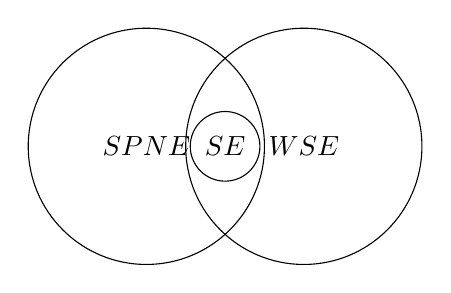
\begin{tikzpicture}
\node[draw, circle] at (0,0) {$SE$};
\node[draw, circle,minimum width=3cm] at (-1,0) {$SPNE$};
\node[draw, circle,minimum width=3cm] at (1,0) {$WSE$};
\end{tikzpicture}  
\end{comment}

\begin{enumerate}

\item 

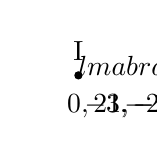
\begin{tikzpicture}
\tikzstyle{mydot} = [circle, minimum width=2pt,fill, inner sep=0pt] % decision node style
\tikzstyle{mystart} = [circle, minimum width=3pt, fill, inner sep=0pt] % starting node style
\tikzset{edge from parent/.style= {draw,  edge from parent path={(\tikzparentnode) -- (\tikzchildnode)}},
 every tree node/.style={mydot}} % make every tree node a decision node; we have to override the start node

\Tree 
    [.\node[mystart, label=above: {I}] {};  
        \edge node[above left] {$l$}; \node[ label=below: {$0,2$}] {}; 
        \edge node[left] {$m$}; [.\node (a) {}; 
            \edge node[left] {$a$}; \node[label=below: {$-3,-1$}] {};  
            \edge node[right] {$b$}; \node[ label=below: {$1,-2$}] {}; ] 
        \edge node[above right] {$r$}; [.\node (b) {};  
            \edge node[left] {$a$}; \node[ label=below: {$-2,-1$}] {};  
            \edge node[right] {$b$}; \node[ label=below: {$3,1$}]  {}; ] ]
\draw[dashed] (a)--node[label=above:II] {}(b);
\end{tikzpicture}

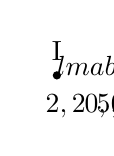
\begin{tikzpicture}
\tikzstyle{mydot} = [circle, minimum width=2pt,fill, inner sep=0pt] % decision node style
\tikzstyle{mystart} = [circle, minimum width=3pt, fill, inner sep=0pt] % starting node style
\tikzset{edge from parent/.style= {draw,  edge from parent path={(\tikzparentnode) -- (\tikzchildnode)}},
 every tree node/.style={mydot}} % make every tree node a decision node; we have to override the start node

\Tree 
    [.\node[mystart, label=above: {I}] {};  
        \edge node[above left] {$l$}; \node[ label=below: {$2,2$}] {}; 
        \edge node[left] {$m$}; [.\node (a) {}; 
            \edge node[left] {$a$}; \node[label=below: {$0,0$}] {};  
            \edge node[right] {$b$}; \node[ label=below: {$5,1$}] {}; ] 
        \edge node[above right] {$r$}; [.\node (b) {};  
            \edge node[left] {$a$}; \node[ label=below: {$0,0$}] {};  
            \edge node[right] {$b$}; \node[ label=below: {$1,3$}]  {}; ] ]
\draw[dashed] (a)--node[label=above:II] {}(b);
\end{tikzpicture}


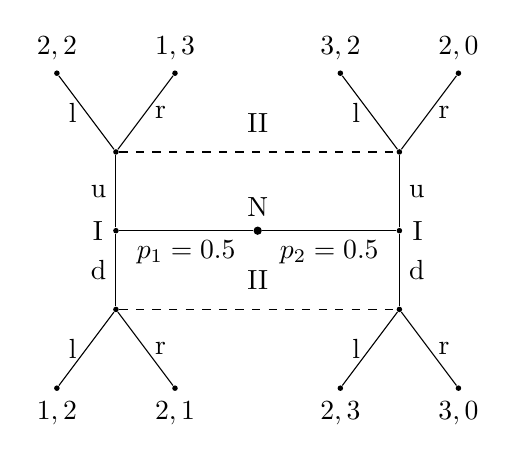
\begin{tikzpicture} % Паук
\tikzstyle{mydot} = [circle, minimum width=2pt,fill, inner sep=0pt] % decision node style
\tikzstyle{mystart} = [circle, minimum width=3pt,fill, inner sep=0pt] % strating node style
\tikzstyle{level 1}=[sibling distance=2cm] % расстояние между соседними узлами на одном уровне
\tikzstyle{level 1}=[level distance=1.8cm] % длина веточки на первом уровне
\tikzstyle{level 2}=[sibling distance=2cm]
\tikzstyle{level 2}=[level distance=1cm]
\tikzstyle{level 3}=[sibling distance=2cm]
\tikzstyle{level 3}=[level distance=1cm]

%
\node[mystart, label=above: {N}] {}
	child[grow=left] {node[mydot, label=left: {I}] {} % left side of the spider
		child[grow=up] {node[mydot] (U1) {} [grow=up]
			child {node[mydot, label=above: {$1,3$}] {}
			edge from parent node[right] {r} }
			child {node[mydot, label=above: {$2,2$}] {}
			edge from parent node[left] {l} }
		edge from parent node[left] {u} }
		child[grow=down] {node[mydot] (D1) {} [grow=down]
			child {node[mydot, label=below: {$1,2$}] {}
			edge from parent node[left] {l} }
			child {node[mydot, label=below: {$2,1$}] {}
			edge from parent node[right] {r} }
		edge from parent node[left] {d} }
    edge from parent node[below] {$p_1=0.5$} }
%
	child[grow=right] {node[mydot, label=right: {I}] {} % right side of the spider
		child[grow=up] {node[mydot] (U2) {} [grow=up]
			child {node[mydot, label=above: {$2,0$}] {}
			edge from parent node[right] {r} }
			child {node[mydot, label=above: {$3,2$}] {}
			edge from parent node[left] {l} }
		edge from parent node[right] {u} }
		child[grow=down] {node[mydot] (D2) {} [grow=down]
			child {node[mydot, label=below: {$2,3$}] {}
			edge from parent node[left] {l} }
			child {node[mydot, label=below: {$3,0$}] {}
			edge from parent node[right] {r} }
		edge from parent node[right] {d} }
    edge from parent node[below] {$p_2=0.5$} } ;
\draw[dashed] (U1)--node[label=above:II] {}(U2);
\draw[dashed] (D1)--node[label=above:II] {}(D2);
\end{tikzpicture}


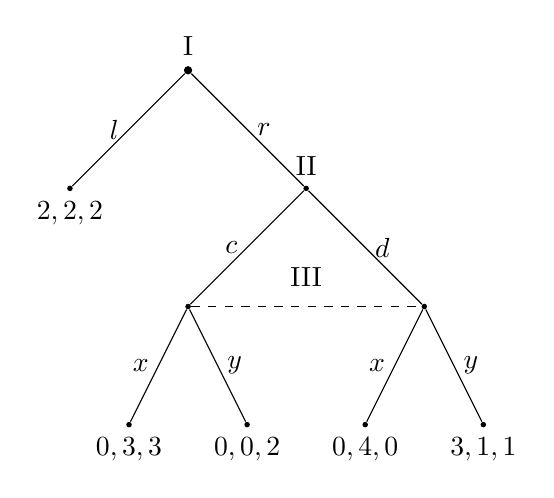
\begin{tikzpicture} % три игрока с выходом первого
\tikzstyle{mydot} = [circle, minimum width=2pt,fill, inner sep=0pt] % decision node style
\tikzstyle{mystart} = [circle, minimum width=3pt,fill, inner sep=0pt] % strating node style
\tikzstyle{level 1}=[level distance=1.5cm] % длина линии
\tikzstyle{level 2}=[level distance=1.5cm] % длина линии
\tikzstyle{level 3}=[level distance=1.5cm] % длина линии
\tikzstyle{level 1}=[sibling distance=3cm] % расстояние между соседними узлами на одном уровне
\tikzstyle{level 2}=[sibling distance=3cm]
\tikzstyle{level 3}=[sibling distance=1.5cm]
\node[mystart, label=above: {I}] {} % создаем узел типа mydot, с пометкой "I" сверху и пустым текстом внутри узла
    child { node[mydot, label=below: {$2,2,2$}] {}        
    edge from parent node[left] {$l$} }
    child { node[mydot, label=above: {II} ] {}        
        child { node[mydot] (a) {} 
                	child {	node[mydot, label=below: {$0,3,3$}] {}
                	edge from parent node[left] {$x$}}
                	child {	node[mydot, label=below: {$0,0,2$}] {}
                	edge from parent node[right] {$y$}  }
        edge from parent node[left] {$c$} }
        child { node[mydot] (b) {}
                	child {	node[mydot, label=below: {$0,4,0$}] {}
                	edge from parent node[left] {$x$}}
                	child {	node[mydot, label=below: {$3,1,1$}] {}
                	edge from parent node[right] {$y$}  }
        edge from parent node[right] {$d$} }
    edge from parent node[right] {$r$} };
\draw[dashed] (a)--node[label=above: {III}] {}(b);
\end{tikzpicture}



\begin{figure}[!htbp]
    \includegraphics{game.28}
\end{figure} 


\begin{figure}[!htbp]
    \includegraphics{game.31}
\end{figure} 


\begin{figure}[!htbp]
    \includegraphics{game.32}
\end{figure} 

Найдите для каждой игры NE, SPNE, WSE и (*) SE 

\item Простейший покер \\
Маша и Саша положили на кон по одному доллар. Маша берет из колоды одну карту. Известно, что выигрышная для Маши карта придет с вероятностью $p$. Маша может либо сразу открыть карту, либо удвоить ставку. Если ставка удвоена, то Саша может либо отказаться от удвоения ставки (и проиграть один доллар), либо поддержать удвоение ставки. Затем карта открывается.
\begin{enumerate}
\item Найдите слабое секвенциальное равновесие в зависимости от $p$ (в чистых и смешанных стратегиях) 
\item Постройте график зависимости цены игры от $p$
\item При каком $p$ игра справедлива, если ставка увеличивается не вдвое, а в $n$  раз?
\item Попробуйте поиграть со своей девушкой (молодым человеком)!
\end{enumerate}

\item Настоящие ковбои заказывают бифштекс!\\
У первого игрока два типа: настоящий ковбой () и сладкоежка ($W$
), которые природа выбирает с вероятностями 0,9 и 0,1 соответственно. Оба игрока знают эти вероятности, но только первый игрок видит ход Природы. Первый игрок делает заказ у стойки бара в тот момент, когда в бар входит второй игрок.\\
Второй игрок - довольно буйный тип. \textit{Тигр: тип не в смысле теории игр, а просто тип.} Он заходит в бар, чтобы подраться, однако он трус и не хотел бы встретиться с настоящим ковбоем. У второго игрока есть выбор: завязывать драку (F) или не завязывать (N). Перед своим ходом второй игрок видит выбор первого игрока. 
Первый игрок может заказать бифштекс (S) или пудинг (P). Настоящие ковбои предпочитают бифштекс, а сладкоежки - пудинг.\\
\begin{figure}[htbp]
    \includegraphics{game.30}
\end{figure} \\
Найдите слабое секвенциальное равновесие.

\item Это война!\\
Две страны, Левая и Правая, хотят поделить территорию в виде отрезка $\left[ {0;1} \right]$. Столицы стран находятся на концах отрезка. Природа выбирает издержки ведения войны:  - для Левой и $c_r $ - для Правой, величины $c_l $ и $c_r $ независимы и равномерно распределены на отрезке $\left[ {0;1} \right]$. Издержки $c_l $ известны только Левой стране. Издержки $c_r $ известны обеим странам. Правая страна выдвигает свои требования к границе $x \in \left[ {0;1} \right]$. Левая страна либо удовлетворяет требования Правой, либо развязывает войну. Правая страна побеждает в войне с экзогенной вероятностью $p \in \left( {0;1} \right)$. Стране-победительнице достается вся территория.\\
\begin{enumerate}
\item Найдите равновесия Нэша в чистых стратегиях; слабые секвенциальные равновесия.
\item Найдите вероятность войны и средние выигрыши игроков в равновесии.
\item Предположим, что издержки ведения войны были бы общеизвестны. Какова была бы вероятность войны и средние выигрыши стран в равновесии?
\item Как изменяться ответы, если требования выдвигает Левая страна?
\end{enumerate}

\item Выкуп доли-2\\
Доля Маши в ЗАО «Красивое платье» составляет $s$, а доля Кати - $\left( {1 - s} \right)$. Маша и Катя решили отказаться от дальнейшего сотрудничества. У ЗАО должна быть одна владелица! Сначала Маша называет цену $p$ - сколько по ее мнению стоит все ЗАО. Затем Катя выбирает выкупить ли за $sp$ Машину долю или продать Маше свою долю за $\left( {1 - s} \right)p$. 
Ценность ЗАО для каждой владелицы – случайная величина равномерная на $\left[ {0;1} \right]$.\\
Найдите равновесие Нэша;

\item Две фирмы производят одинаковый продукт. Сначала первая фирма выбирает свой объем выпуска, $q_1$. Затем вторая фирма, зная $q_1$, выбирает свой объем выпуска, $q_2$. Предельные издержки выпуска первой фирмы равны $1$ и общеизвестны. Предельные издержки второй фирмы равновероятно равны $1$ или $2$. Вторая фирма точно знает, чему равны ее предельные издержки. Первая фирма знает только возможные значения издержек второй фирмы и их вероятности. Каждая фирма максимизирует свою прибыль. Обратная функция спроса имеет вид $p=10-q$. 
\begin{enumerate}
\item Найдите равновесие Нэша, совершенное в подыграх
\item Какие объемы выпуска будут выбирать фирмы в найденном равновесии?
\end{enumerate}

\end{enumerate}

\section{Дополнительные задачи}

\begin{enumerate}


\item Заработок короля\\
В стране  $n$  жителей, каждый из которых получает заработную плату в одну монету. Когда в стране победила демократия, король потерял свою власть, даже был лишен права голоса. Единственное, что он может - так это предлагать перераспределение заработной платы. Зарплата каждого жителя должна выражаться неотрицательным количеством монет, в сумме все зарплаты должны равняться  $n$ . Когда король предлагает перераспределение зарплаты, каждый житель, кроме самого короля, может проголосовать за, против или вообще не приходить на голосование. Новое распределение одобряется, если число голосов <<за>> строго больше числа голосов <<против>>.\\
Каждый житель эгоистичен, голосует <<за>>, если в новом проекте его зарплата растет, <<против>>, если падает, и не приходит на голосование, если ему предлагается одинаковая зарплата.\\
Какую зарплату в результате получит хитрый король и сколько голосований ему потребуется?

\item (*) Покер в чате\\
Трое заядлых игроков в покер сидят в чате. Предложите процедуру раздачи карт, при которой каждый игрок знает свои карты и не знает карт соперника. Игроки абсолютно рациональны и обладают безграничными вычислительными возможностями, поэтому использование кодов с открытым ключом (типа RSA) недопустимо. В чате можно посылать сообщения, адресованные как всем сразу, так и конкретному лицу.

\item Игры с моделью Кидленда-Прескотта \\
Правительство пообещало, что инфляция будет равна нулю в следующем году! После сенсационного объявления народ определяет свои ожидания инфляции $\pi ^e $. Зная ожидания народа, правительство выбирает фактический уровень инфляции $\pi $ в будущем году. Функция полезности правительства $U =  - \left( {\pi  - \pi ^p } \right)^2  - \left( {y - y^p } \right)^2 $
, где $y^p $ - желаемый правительством уровень выпуска, а $\pi ^p  > 0$ - желаемый правительством уровень инфляции. \\
Совокупное предложение задано функцией $y = y^{*}  + b\left( {\pi  - \pi ^e } \right)$, где $y^{*}$ - потенциальный уровень выпуска. Константа $b$ - положительная.\\
Найдите равновесие Нэша и платежи, получаемые игроками в следующих ситуациях:
\begin{enumerate}
\item Население верит правительству, а правительство не обязано исполнять свои обязательства.
\item Население верит правительству, а правительство исполняет свои обязательства.
\item Функция полезности населения имеет вид $U =  - \left( {\pi  - \pi ^e } \right)^2 $, а правительство исполняет свои обязательства. Тигр: С такой функцией полезности население догадается!
\item Функция полезности населения имеет вид $U =  - \left( {\pi  - \pi ^e } \right)^2 $, а правительство не обязано исполнять свои обязательства.
\item Какой должна быть величина штрафа за неисполнение обязательств, чтобы в пункте г) правительство было заинтересовано в их исполнении?
\item Сравните выигрыш правительства в случаях <<в>> и <<г>>. Обратите внимание на то, что в случае <<в>> у правительства нет возможности нарушать обещание, а в случае <<г>> такая возможность появляется.
\end{enumerate}

\item Передача информации в модели Курно.\\
Две фирмы по очереди выбирают объемы производства. Вторая фирма при выборе своего объема производства не знает объема, выбранного первой фирмой. После того, как обе фирмы произвели товар, рынок определяет цены в соответствии с функцией спроса $P\left( Q \right) = 1 - Q$
, где $Q = q_1  + q_2 $.
\begin{enumerate}
\item Что представляет собой стратегия второй фирмы? Найдите равновесие Нэша. Совпадает ли оно с равновесием Нэша совершенным в подыграх?
\item Предположим теперь, что первая фирма честно декларирует выбранный ею объем выпуска. Что представляет собой стратегия второй фирмы? Найдите равновесие Нэша, совершенное в подыграх. Будут ли другие равновесия Нэша?
\item Сравните платежи второй фирмы в обоих вариантах модели. Почему наличие дополнительной информации снижает платеж второй фирмы? Почему не корректно рассуждение <<Полученную информацию можно не учитывать, поэтому платеж не может упасть>>?
\end{enumerate}

\item (*) Пираты делят золото \\
Есть золотой песок и три пирата, но нет весов.\\
Предпочтения пиратов субъективны (действительно равные кучи могут казаться пирату неравными). Но предпочтения стабильны: если пират считал две кучи равными,  и видит, что к первой досыпали песок, то он будет считать первую кучу большей. Каждый пират может делить кучу песка на равные кучи, сравнивать несколько куч, отсыпать из большей кучи песок так, чтобы она сравнялась с меньшей.\\
Предложите конечную процедуру справедливого дележа, при которой у пиратов не было бы зависти (каждый считал бы, что его часть не меньше, чем у других).

\item Футбол\\
Четыре команды играют в футбол. Сначала проводится полуфинал (первая команда играет со второй, третья - с четвертой), затем две команды победительницы участвуют в финале. Выигравшая чемпионат команда получает приз равный  $S$ . Перед началом чемпионата каждая команда выбирает затраты на тренировки  $a$  (неотрицательное число). Если встречаются команды с затратами  $a$  и  $b$ , то вероятность выигрыша первой равна  $\frac{a}{a+b} $ .\\
{\it Тигр: А может быть это фирмы дают взятки чиновникам?}
\begin{enumerate}
\item Найдите симметричное  равновесие  Нэша (т.е. равновесие в котором все команды выбирают одинаковый уровень усилий);
\item Пусть команд будет восемь, а игра проходит по схеме четвертьфинал-полуфинал-финал. Докажите, что симметричного равновесия Нэша не существует.\\
{\it Тигр: А если вторая производная  окажется равной нулю?}\\
{\it  Автор: Тсс!}
\item Докажите, что симметричное равновесие Нэша отсутствует, если число туров превышает два.
\item (*) Докажите, что если число туров превышает два, то в любом равновесии Нэша будет команда с нулевым уровнем тренировки.\\
{\it Тигр: Среди кандидатов в президенты есть те, кто не надеется победить, среди студентов есть те, кто не готовится к экзамену... Все это звенья одной цепи!}
\end{enumerate}

\item (*) Русская рулетка \\
Два гусара, одна дама, одна пуля в шестизарядном револьвере...\\
Сначала первый гусар выбирает, отправиться ли ему в кабак (тогда он получит полезность ноль, а дама достанется другому) или приставить револьвер к виску и нажать на курок. Смерть означает полезность равную минус единице (при этом дама, естественно, достается другому). Если гусар остается жив, то право и обязанность выбора кабак/стреляться переходит ко второму. Барабан револьвера при этом не перекручивается, т.е. вероятность смерти увеличивается. Ценность дамы для одного гусара  $a$ , для другого -  $b$ .
\begin{enumerate}
\item Найдите равновесия в зависимости от  $a$  и  $b$ .
\item Каким игроком лучше быть, первым или вторым, в зависимости от   $a$  и  $b$ .
\end{enumerate}
{\it Тигр: Настоящего джентльмена, конечно, интересует настоящая дама, } $a\gg 1$, $b\gg 1$ 

\item Limbo \\
До весны 2007 года в Швеции существовала необычная лотерея <<Limbo>>. Правила выглядят следующим образом. Вы можете выбрать любое натуральное число. Победителем объявляется тот, кто назвал самое маленькое число, никем более не названное. Например, если игроки назвали числа 1, 3, 1, 2, 4, то победителем будет тот, кто назвал число 2. 
\begin{enumerate}
\item Опишите все равновесия Нэша в чистых стратегиях для $n$ игроков 
\item Найдите симметрическое равновесие для трех игроков (т.е. равновесие, в котором все игроки используют одинаковые стратегии) 
\item Почему была закрыта эта лотерея? 
\end{enumerate}
Подсказка: какие есть известные законы распределения на $\mathbb{N}$? 

\item (**) Continuous Colonel Blotto \\
Two generals have the same amount of units (continuous) to compete over three battlefields in a campaign. In each battlefield, the general who assigns more units wins. The general winning 2 battlefields wins the entire campaign. They simultaneously announce their decision of unit distribution over the three battlefields. Find NE \\
Hint1: is it possible that $U_{1}+U_{2}+U_{3}=1$ and $U_{i}$ - uniform? \\
Hint2: сумма высот проведенных из точки $N$ к трем сторонам треугольника не зависит от выбора точки $N$ 

\item (*) Петя выбирает место где спрятаться внутри круга единичного радиуса. Одновременно Вася выбирает место, где будет искать Петю. Вася замечает Петю, если расстояние между ними не превосходит половины радиуса. Если Вася нашел Петю, то Петя платит Васе рубль. Если Вася не нашел Петю, то Вася - Пете. \\
Найдите цену игры. 

\end{enumerate}

\section{Варианты контрольных} 

\subsection{Контрольная номер 1. 2007.} 
\begin{enumerate}
\item В игре участвуют три игрока. Сначала первый игрок выбирает $x\in R$; затем второй игрок, зная $x$, выбирает $y\in R$; затем третий игрок, зная $x$ и $y$, выбирает $z\in \left[1;2\right]$. Функции выигрыша имеют вид: \\
$U_{1} =xyz+\frac{9x}{z} -zx^{2}$ \\
$U_{2} =\left(z-2\right)y^{2} -4xy+\left(5+z\right)y+5x$\\
$U_{3} =2x^{3} -y^{4} -3z-z^{2}$  \\
Какие $x$, $y$ и $z$ будут реализованы игроками при использовании ими метода обратной индукции? \\
Ответ: $x=2$, $y=-1$ и $z=1$ 

\item Найдите равновесие в смешанных стратегиях и цену игры в матричной игре с противоположными интересами: \\
$
\begin{array}{c|cccc}
& b_1 & b_2 & b_3 & b_4 \\
\hline
a_1 & 1 & 12 & -10 & -8 \\
a_2 & -9 & -10 & 2 & -4 \\
\end{array}
$ \\
Ответ: $p=5/14$, $v=-38/7$, $q_{1}=2/7$, $q_{4}=5/7$ 

\item Найдите равновесные Нэша исходы (в чистых и смешанных стратегиях) и Парето оптимальные исходы (в чистых стратегиях) следующих биматричных игр:\\
a) 
$\begin{array}{c|ccc} 
& d & e & f\\
\hline
a & (1;2) & (4;4) & (-4;3) \\
b & (4;3) & (1;0) & (2;1) \\
c & (2;3) & (6;6) & (3;7) \\
\end{array}$ 
б) 
$\begin{array}{c|ccc} 
& d & e & f\\
\hline
a & (3;-1) & (1;5) & (4;1) \\
b & (2;1) & (-1;7) & (5;0) \\
c & (1;5) & (1;-1) & (5;1) \\
\end{array}$ \\
Ответ: \\
а) NE: $(b,d)$, $(c,f)$, $(\frac{2}{3}b+\frac{1}{3}c,\frac{1}{3}d+\frac{2}{3}f)$ \\
PO: $(6;6)=(c,e)$, $(3;7)=(c,f)$ \\
б) NE $(ta+(1-t)c,e)$, где $t\in[\frac{1}{2},1]$ \\
PO: $(5;1)=(c,f)$, $(1;5)=(c,d)$, $(1;5)=(a,e)$, $(-1;7)=(b,e)$ \\
В этом пункте вычеркивание начинается с $\frac{1}{2}d+\frac{1}{2}e\succ f$ 

\item На рисунке представлена последовательная игра двух игроков: I и II. \\
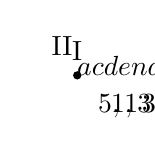
\begin{tikzpicture}
\tikzstyle{mydot} = [circle, minimum width=2pt,fill, inner sep=0pt] % decision node style
\tikzstyle{mystart} = [circle, minimum width=3pt, fill, inner sep=0pt] % starting node style
\tikzset{edge from parent/.style= {draw,  edge from parent path={(\tikzparentnode) -- (\tikzchildnode)}},
 every tree node/.style={mydot}} % make every tree node a decision node; we have to override the start node

\Tree 
    [.\node[mystart, label=above: {I}] {};  
        \edge node[above left] {$a$}; [.\node[ label=above left:II] {}; 
            \edge node[left] {$c$}; [.\node (a) {};  
                \edge node[left] {$d$}; \node[ label=below: {$5,1$}] {}; 
                \edge node[right] {$e$}; \node[ label=below: {$1,3$}] {}; ]   
            \edge node[right] {$n$}; [.\node (b) {};  
                \edge node[left] {$d$}; \node[ label=below: {$3,0$}] {}; 
                \edge node[right] {$e$}; \node[ label=below: {$4,3$}] {}; ]   ]
        \edge node[above right] {$b$}; [.\node[ label=above right:II] {};  
            \edge node[left] {$f$}; \node[ label=below: {$4,2$}] {};  
            \edge node[right] {$g$}; \node[ label=below: {$4,1$}] {}; ] ]
\draw[dashed] (a)--node[label=above:I] {}(b);
\end{tikzpicture}

\begin{enumerate}
\item Представьте игру в нормальной (матричной) форме 
\item Найдите все равновесия Нэша (в чистых стратегиях)
\item Найдите все равновесия Нэша, совершенные в подыграх (в чистых стратегиях) 
\end{enumerate}
Ответ: \\
б) NE: $(ad,cf)$, $(ad,cg)$, $(ae,nf)$, $(ae,ng)$, $(bd,nf)$, $(be,nf)$ \\
в) SPNE: $(ad,cf)$, $(ae,nf)$, $(be,nf)$ 

\item	На столе лежат $n$ фишек. Два игрока (Саша и Маша) по очереди убирают некоторое количество фишек. Саша может убрать либо 1, либо 2 фишки. Маша может убрать либо 3, либо 4 фишки. Проигрывает тот, кто не сможет сделать очередной ход. Кто победит в следующих четырех случаях, если игроки при выборе стратегий используют метод обратной индукции? \\
a) Первым ходит Саша, $n=132$  \\
б) Первым ходит Саша, $n=175$  \\
в) Первой ходит Маша, $n=132$  \\
г) Первой ходит Маша, $n=175$  \\
Ответ: \\
а) Саша \\
б) Маша \\
в) Саша \\
г) Саша \\
\end{enumerate}

\subsection{Контрольная номер 2. 2007.} 
\begin{enumerate}
\item Саша и Маша поссорились и предпочитают развлекаться отдельно друг от друга. Матрица игры имеет вид: \\
$\begin{array}{c|cc}
& $Футбол$ & $Балет$ \\
\hline
$Футбол$ & (0;0) & (2+t_{1};2) \\
$Балет$ & (1;3+t_{2}) & (0;0)\\
\end{array}$\\
В матрице Саша - первый игрок, Маша - вторая. \\
Величина $t_1$ известна Саше, но неизвестна Маше. Величина $t_2$ известна Маше, но неизвестна Саше. Обоим известно, что $t_1$ и $t_2$ - случайные величины, равномерно распределенные на промежутках $[0;12]$ и $[0;7]$ соответственно. \\
Найдите разделяющее Байесовское равновесие $(s, m)$, для которого: \\
Саша выбирает Футбол, если $t_{1}>s$, и Балет в противном случае, \\
а Маша выбирает Футбол, если $t_{2}>m$, и Балет в противном случае. \\
Ответ: $(4;1)$, $7-3m=sm$, $24-5s=sm$ 

\item Задана бесконечно повторяемая игра $G(\infty;\delta)$ \\
$\begin{array}{c|cc}
& t_{2} & t_{2} \\
\hline
s_{1} & (2;1) & (6;-2) \\
s_{2} & (0;5) & (4;2) \\
\end{array}$
a) Сформулируйте стратегии переключения, при которых игроки будут играть $(s_2;t_2)$ во всех партиях \\
б) При каких значениях $\delta$ эти стратегии составляют совершенное подыгровое равновесие Нэша? \\
Ответ: \\
а) Для первого игрока: \\
В первой партии сделать ход $s_{2}$ \\
В $n$-ой партии ($n\ge2$) сделать ход $s_{2}$, если во всех предыдущих партиях был сыгран исход $(s_{2};t_{2})$; иначе сделать ход $s_{1}$ \\
б) $\delta\in [0.75;1)$ 

\item Два игрока одновременно выбирают действительные числа $x_{1}$ и $x_{2}$  соответственно. Платежные функции игроков могут иметь один из двух видов: \\
$\left\{
\begin{array}{c}
U_{1}=-x_{1}^{2}-x_{1}x_{2}+2x_{1} \\
U_{2}=-x_{2}^{2}+2x_{1}x_{2}-x_{2}
\end{array}\right.$ с вероятностью 0,8;\\
$\left\{
\begin{array}{c}
U_{1}=-x_{1}^{2}+2x_{1}x_{2}+3x_{1} \\
U_{2}=-x_{2}^{2}+x_{1}x_{2}+x_{2}
\end{array}\right.$ с вероятностью 0,2;\\
Первый игрок точно знает, какой вид имеют платежные функции. Оба игрока знают законы распределения. Найти равновесие Нэша в чистых стратегиях.\\
Ответ: $x_{1a}=\frac{3}{4}$, $x_{1b}=2$, $x_{2}=\frac{1}{2}$ 

\item Найдите слабые секвенциальные равновесия в чистых стратегиях в игре: \\

\begin{figure}[htbp]
    \includegraphics{game.39}
\end{figure}
Ответ: $\left\{(lL,uD); p=0.2; q\in [0;1]\right\}$, $\left\{(rR,dD);p\ge \frac{1}{4} ;q=0.2\right\}$

\item Найдите слабые секвенциальные равновесия в чистых стратегиях в игре: \\

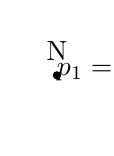
\begin{tikzpicture}
\tikzstyle{mydot} = [circle, minimum width=2pt,fill, inner sep=0pt] % decision node style
\tikzstyle{mystart} = [circle, minimum width=3pt, fill, inner sep=0pt] % starting node style
\tikzset{edge from parent/.style= {draw,  edge from parent path={(\tikzparentnode) -- (\tikzchildnode)}},
 every tree node/.style={mydot}} % make every tree node a decision node; we have to override the start node

\Tree 
    [.\node[mystart, label=above: N] {};  
        \edge node[above left] {$p_1=0.3$}; [.\node (c) {}; 
            \edge node[left] {$a$}; \node[ label=below: {$4,2$}] {}; 
            \edge node[right] {$b$}; \node[ label=below: {$3,1$}] {}; ] 
        \edge node[above right] {$p_2=0.2$}; [.\node (d) {};  
            \edge node[left] {$a$}; \node[ label=below: {$2,3$}] {};  
            \edge node[right] {$b$}; [.\node (b) {}; 
                \edge node[left] {$c$}; \node[ label=below: {$5,4$}] {}; 
                \edge node[right] {$d$}; \node[ label=below: {$2,0$}] {}; ]   ]   
        \edge node[above left] {$p_3=0.5$}; [.\node (a) {}; 
            \edge node[left] {$c$}; \node[ label=below: {$3,1$}] {}; 
            \edge node[right] {$d$}; \node[ label=below: {$0,2$}] {}; ] ]
\draw[dashed] (a)--node[label=above:II] {}(b);
\draw[dashed] (c)--node[label=above:I] {}(d);
\end{tikzpicture}


\begin{figure}[htbp]
    \includegraphics{game.40}
\end{figure}

Ответ: $\left\{(a,d); \mu=\frac{3}{5}; \nu=0\right\}$, 
$\left\{(b,c); \mu=\frac{3}{5}; \nu=\frac{2}{7}\right\}$
\end{enumerate}

\subsection{Контрольная номер 1. 2011.} 
\begin{enumerate}

\item Найти равновесие в смешанных стратегиях и цену игры в матричной игре с противоположными интересами

\begin{tabular}{c|cccc}
 & a & b & c & d \\ 
\hline 
q & -3 & -2 & 5 & 1 \\ 
e & 2 & 0 & -2 & -2 \\ 
r & 6 & 2 & -5 & -3 \\ 
\end{tabular} 



Решая неравенства обнаруживаем, что строго доминируется стратегия $e$. (3 балла)

Ответ: $p_{I}=(\frac{5}{8};0;\frac{3}{8})$ (3 балла), $p_{II}=(0;\frac{1}{2};0;\frac{1}{2})$ (3 балла), $v=-0{,}5$ (1 балл).

\item Найдите равновесные по Нэшу исходы (в чистых и смешанных стратегиях) и Парето оптимальные точки (в чистых стратегиях) в биматричной игре

\begin{tabular}{c|ccc}
 & c & d & e \\ 
\hline 
a & 3;3 & 0;1 & 2;3 \\ 
b & 1;0 & 2;3 & 1;2 \\ 
\end{tabular} 


NE: Чистые: $(a,c)$, $(b,d)$, $(a,e)$ (2 балла), Парето: $(3;3)$ (1 балл) \\
смешанные: $(\frac{1}{3}a+\frac{2}{3}b,\frac{1}{3}d+\frac{2}{3}e)$, $(a,qc+(1-q)e)$ где $q\in [0;1]$ (7 баллов). 

\item Игрок A выбирает действительное число $x\in [-3;2]$, а игрок B одновременно с ним число $y\in [-2;4]$. Найдите равновесие Нэша. Функции выигрыша игроков: $u_A=-x^2-6xy+26x$, $u_B=-y^2+4xy-6y$.

Ответ: $(x=2;y=1)$ (10 баллов)

\item На столе лежит $N$ фишек. Два игрока (Саша и Маша) по очереди убирают некоторое количество фишек. Саша может убрать либо 1, либо 3 фишки. Маша может убрать либо 2, либо 4 фишки. \textbf{Выигрывает} тот, кто не сможет сделать очередной ход. Кто победит в следующих четырех случаях, если игроки при выборе стратегий используют метод обратной индукции? (Заполнитe таблицу ответов – в пустые клетки проставить имя победителя)?

\begin{tabular}{c|cc}
 & $N=321$ & $N=383$ \\ 
\hline 
Первым ходит Саша &  &  \\ 
Первой ходит Маша &  &  \\ 
\end{tabular} 



Таблица с плюсами и минусами (5 баллов): \\
\begin{tabular}{c|cc}
 & Маша & Саша \\ 
\hline 
1 & -- & + \\ 
2 & -- & -- \\ 
3 & + & + \\ 
4 & -- & + \\ 
5 & + & + \\ 
6 & -- & + \\ 
7 & -- & -- \\ 
8 & + & + \\ 
9 & -- & + \\ 
10 & + & + \\ 
\end{tabular} 

Итоговая таблица (5 баллов): \\
\begin{tabular}{c|cc}
 & $N=321$ & $N=383$ \\ 
\hline 
Первым ходит Саша & Маша & Саша \\ 
Первой ходит Маша & Маша &  Маша \\ 
\end{tabular} 


Штраф за решение противоположной задачи: 2 балла.

\item На рисунке представлена последовательная игра двух игроков с участием природы. Представить ее в нормальной форме (построить матричную игру), найти все Нэш-равновесия (NE) в чистых стратегиях и равновесия, совершенные в подыграх (SPNE) в чистых стратегиях.  


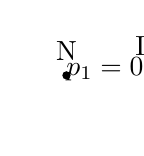
\begin{tikzpicture}
\tikzstyle{mydot} = [circle, minimum width=2pt,fill, inner sep=0pt] % decision node style
\tikzstyle{mystart} = [circle, minimum width=3pt, fill, inner sep=0pt] % starting node style
\tikzset{edge from parent/.style= {draw,  edge from parent path={(\tikzparentnode) -- (\tikzchildnode)}},
 every tree node/.style={mydot}} % make every tree node a decision node; we have to override the start node

\Tree 
    [.\node[mystart, label=above: {N}] {};  
        \edge node[above left] {$p_1=0.5$}; [.\node[ label=above left:I] {}; 
            \edge node[left] {$a$}; \node[label=below: {$5,1$}] {};  
            \edge node[right] {$b$}; [.\node[ label=above right:II] {};  
                \edge node[left] {$m$}; \node[ label=below: {$1,2$}] {}; 
                \edge node[right] {$n$}; \node[ label=below: {$2,3$}] {}; ]   ]
        \edge node[above right] {$p_2=0.5$}; [.\node[ label=above right:II] {};  
            \edge node[left] {$c$}; [.\node (a) {};  
                \edge node[left] {$z$}; \node[ label=below: {$1,0$}] {}; 
                \edge node[right] {$t$}; \node[ label=below: {$2,2$}] {}; ] 
            \edge node[right] {$d$}; [.\node (b) {}; 
                \edge node[left] {$z$}; \node[ label=below: {$3,1$}] {}; 
                \edge node[right] {$t$}; \node[ label=below: {$0,0$}] {}; ]   ]   ]
\draw[dashed] (a)--node[label=above:I] {}(b);
\end{tikzpicture}

Ответ: NE: $(at,cm)$, $(at,cn)$, $(az,dm)$, $(az,dn)$;  SPNE: $(at,cn)$, $(az,dn)$ 


Составление матрицы -- 4 балла, поиск NE -- 2 балла, поиск SPNE -- 4 балла.

\item У журнала 2011 читателей. Журнал предлагает читателям игру. Каждый читатель имеет возможность отправить смс на специальный номер. Если журнал получает только одно смс, то его отправитель получает приз 1000 рублей. Если журнал получает больше одного смс, то никто из читателей не получает ничего. Стоимоcть отправки смс 1рубль
\begin{enumerate}
\item Найдите все чистые равновесия Нэша;
\item Найдите симметричное равновесие Нэша в смешанных стратегиях;
\item Сколько в среднем выигрывает редакция журнала в указанном смешанном равновесии?
\end{enumerate}
Решение.
\begin{enumerate}
\item (2 балла) Чистые: ровно один читатель отправляет смс, остальные 2010 не отправляют.
\item (4 балла) Пусть каждый читатель кроме первого отправляет смс с вероятностью $p$. Чтобы первому игроку было оптимально использовать смешанную стратегию он должен быть безразличен между чистыми.

Если читатель не отправляет смс, то он получает ноль. Если он отправляет смс, то выигрывает только в случае если никто другой не отправит смс (вероятность $(1-p)^{2010}$) 
\begin{equation}
\label{eq_foc}
-1+1000\cdot (1-p)^{2010}=0
\end{equation}
Отсюда $p=1-(1/1000)^{1/2010}$.

\item (4 балла) Средний выигрыш редакции равен
\begin{equation}
U_{R}=2011p-1000(2011p(1-p)^{2010})=0
\end{equation}
\end{enumerate}


\end{enumerate}

\subsection{Контрольная номер 2. Усредненная версия. 2011.} 

\begin{enumerate}
\item Рассмотрим бесконечно повторяемую игру с дисконт-фактором $\delta$ и матрицей

\begin{equation}
\begin{array}{c|cc}
 & c & d \\ 
\hline
c & 3;3 & 0;6 \\ 
d & 6;0 & 2;2
\end{array} 
\end{equation}

\begin{enumerate}
\item Сформулируйте стратегии жесткого переключения для каждого игрока?
\item При каких $\delta$ указанный профиль стратегий будет равновесием Нэша?
\item Равновесием Нэша совершенным в подыграх?
\item Как изменятся ответы на (b) и (c), если в правой верхней ячейке матрицы, $cd$, будет находится вектор выигрышей $6;0$?
\end{enumerate}


\item Две фирмы производят одинаковый продукт. Они одновременно выбирают свои объемы выпуска, $q_1$ и $q_2$. Предельные издержки выпуска первой фирмы равны $1$ и общеизвестны. Предельные издержки второй фирмы равновероятно равны $0$ или $3$. Вторая фирма точно знает, чему равны ее предельные издержки. Первая фирма знает только возможные значения издержек второй фирмы и их вероятности. Каждая фирма максимизирует свою прибыль. Обратная функция спроса имеет вид $p=14-q$, где $q=q_1+q_2$ --- общий выпуск фирм. Найдите равновесие Нэша.

\item Маша и Саша спорят на деньги, кто лучше сдаст теорию игр. Для простоты будем считать, что одинаковый итоговый балл невозможен. Маша и Саша одновременно делают ставки в деканате: один или два рубля. Уровень знаний Маши --- случайная величина, $M$, равномерная на отрезке $[0;1]$. Уровень знаний Саши --- случайная величина, $S$, равномерная на отрезке $[0;1]$. Маша знает $M$, Саша знает $S$, величины $M$ и $S$ независимы. Вероятность того, что Маша наберет больше баллов по теории игр равна $M/(M+S)$. Тот, кто набирает больше баллов получает обе ставки. Проигравший теряет свою ставку. 

Найдите равновесие Нэша в этой игре. Если при нахождении параметров равновесия возникает <<неберущееся>> уравнение, не решайте его --- достаточно выписать это уравнение и аккуратно сформулировать стратегию каждого игрока.


\end{enumerate}


\subsection{Экзамен. 2011.} 

\begin{enumerate}
\item Две фирмы производящие идентичный товар одновременно выбирают объем выпуска. Предельные издержки фирм равны 2 и 3 соответственно. Обратная функция спроса на продукцию имеет вид $P=50-Q$, где $Q$ --- совокупный выпуск двух фирм, $Q=Q_1+Q_2$.
\begin{enumerate}
\item Найдите равновесие Нэша в статической игре
\item Верно ли, что профиль стратегий $S=\{Q_1=12,Q_2=12\}$ доминирует по Парето найденное равновесие Нэша?
\end{enumerate}
Рассмотрите игру, где указанная статическая игра двух фирм повторяется бесконечное количество раз с дисконт-фактором $\delta$. 
\begin{enumerate}
\item[(c)] Сформулируйте стратегии жесткого переключения при применении которых в каждой базовой игре играется исход $S$
\item[(d)] При каких $\delta$ сформулированные стратегии жесткого переключения будут равновесием Нэша
\end{enumerate}


\item Саша и Маша играют в статическую игру. Саша выбирает одни из двух строк. Маша выбирает один из двух столбцов. Матрица выигрышей имеет вид А с вероятностью $0{,}2$ и вид B с вероятностью $0{,}8$. Маша знает точно, какой вид имеет матрица игры, Саша --- не знает. Найдите равновесие Нэша.


\begin{tabular}{c|cc}
A & c & d \\ 
\hline 
a & $3,0$ & $0,2$ \\ 
b & $0,2$ & $2,1$ \\ 
\end{tabular} 


\begin{tabular}{c|cc}
B & c & d \\ 
\hline 
a & $0,3$ & $4,0$ \\ 
b & $3,-1$ & $1,2$ \\ 
\end{tabular} 



\item Найдите все слабые секвенциальные равновесия в чистых стратегиях


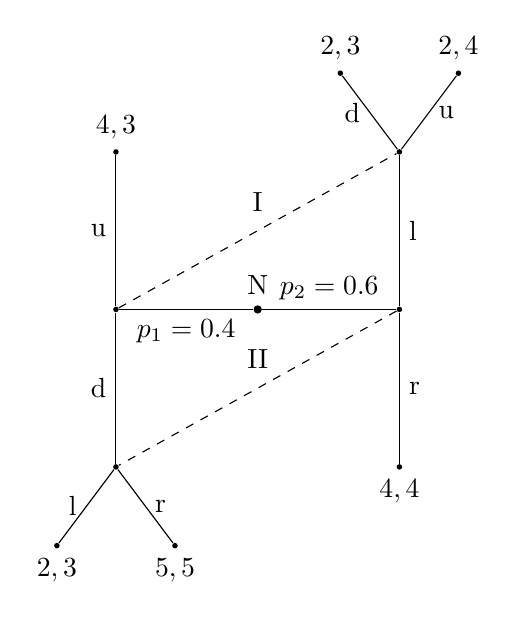
\begin{tikzpicture} % укороченный паук
\tikzstyle{mydot} = [circle, minimum width=2pt,fill, inner sep=0pt] % decision node style
\tikzstyle{mystart} = [circle, minimum width=3pt,fill, inner sep=0pt] % strating node style
\tikzstyle{level 1}=[sibling distance=2cm] % расстояние между соседними узлами на одном уровне
\tikzstyle{level 1}=[level distance=1.8cm] % длина веточки на первом уровне
\tikzstyle{level 2}=[sibling distance=2cm]
\tikzstyle{level 2}=[level distance=2cm]
\tikzstyle{level 3}=[sibling distance=2cm]
\tikzstyle{level 3}=[level distance=1cm]

%
\node[mystart, label=above: {N}] {}
	child[grow=left] {node[mydot] (ia) {} % left side of the spider
		child[grow=up] {node[mydot,label=above: {$4,3$}] {} [grow=up] 
		edge from parent node[left] {u} }
		child[grow=down] {node[mydot] (iib) {} [grow=down]
			child {node[mydot, label=below: {$2,3$}] {}
			edge from parent node[left] {l} }
			child {node[mydot, label=below: {$5,5$}] {}
			edge from parent node[right] {r} }
		edge from parent node[left] {d} }
    edge from parent node[below] {$p_1=0.4$} }
%
	child[grow=right] {node[mydot] (iia) {} % right side of the spider
		child[grow=up] {node[mydot] (ib) {} [grow=up]
			child {node[mydot, label=above: {$2,4$}] {}
			edge from parent node[right] {u} }
			child {node[mydot, label=above: {$2,3$}] {}
			edge from parent node[left] {d} }
		edge from parent node[right] {l} }
		child[grow=down] {node[mydot,label=below: {$4,4$}] {} [grow=down] 
		edge from parent node[right] {r} }
    edge from parent node[above] {$p_2=0.6$} } ;
\draw[dashed] (ia)--node[label=above:I] {}(ib);
\draw[dashed] (iia)--node[label=above:II] {}(iib);
\end{tikzpicture}



\item Найдите все слабые секвенциальные равновесия в чистых стратегиях


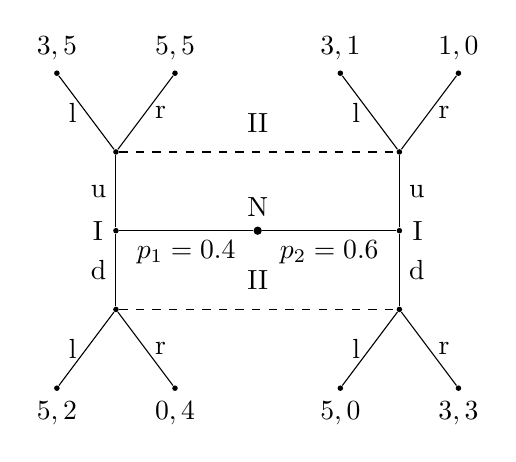
\begin{tikzpicture} % Паук
\tikzstyle{mydot} = [circle, minimum width=2pt,fill, inner sep=0pt] % decision node style
\tikzstyle{mystart} = [circle, minimum width=3pt,fill, inner sep=0pt] % strating node style
\tikzstyle{level 1}=[sibling distance=2cm] % расстояние между соседними узлами на одном уровне
\tikzstyle{level 1}=[level distance=1.8cm] % длина веточки на первом уровне
\tikzstyle{level 2}=[sibling distance=2cm]
\tikzstyle{level 2}=[level distance=1cm]
\tikzstyle{level 3}=[sibling distance=2cm]
\tikzstyle{level 3}=[level distance=1cm]

%
\node[mystart, label=above: {N}] {}
	child[grow=left] {node[mydot, label=left: {I}] {} % left side of the spider
		child[grow=up] {node[mydot] (U1) {} [grow=up]
			child {node[mydot, label=above: {$5,5$}] {}
			edge from parent node[right] {r} }
			child {node[mydot, label=above: {$3,5$}] {}
			edge from parent node[left] {l} }
		edge from parent node[left] {u} }
		child[grow=down] {node[mydot] (D1) {} [grow=down]
			child {node[mydot, label=below: {$5,2$}] {}
			edge from parent node[left] {l} }
			child {node[mydot, label=below: {$0,4$}] {}
			edge from parent node[right] {r} }
		edge from parent node[left] {d} }
    edge from parent node[below] {$p_1=0.4$} }
%
	child[grow=right] {node[mydot, label=right: {I}] {} % right side of the spider
		child[grow=up] {node[mydot] (U2) {} [grow=up]
			child {node[mydot, label=above: {$1,0$}] {}
			edge from parent node[right] {r} }
			child {node[mydot, label=above: {$3,1$}] {}
			edge from parent node[left] {l} }
		edge from parent node[right] {u} }
		child[grow=down] {node[mydot] (D2) {} [grow=down]
			child {node[mydot, label=below: {$5,0$}] {}
			edge from parent node[left] {l} }
			child {node[mydot, label=below: {$3,3$}] {}
			edge from parent node[right] {r} }
		edge from parent node[right] {d} }
    edge from parent node[below] {$p_2=0.6$} } ;
\draw[dashed] (U1)--node[label=above:II] {}(U2);
\draw[dashed] (D1)--node[label=above:II] {}(D2);
\end{tikzpicture}


\end{enumerate}



\newpage
\textbf{Названия некоторых стратегий в повторяющейся дилемме заключенного }\\

$\begin{array}{c|cc}
 & c & d \\
\hline
c & 5;5 & 0;6 \\
d & 6;0 & 3;3 \\
\end{array}$ \\
Стратегия $d$ строго доминирует стратегию $c$, однако (c;c) - одна из Парето оптимальных точек. \\


{\bf Всегда <<c>>} \\
В любой партии делать ход c независимо от предыстории. \\
{\bf Всегда <<d>>} \\
В любой партии делать ход d независимо от предыстории. \\
{\bf Цикл <<ccd>>} \\
В первой партии сделать ход c, во второй - c, в третьей d, далее снова играется c, c, d... \\
{\bf Стратегия переключения} (grim trigger)\\
В первой партии cделать ход c. В $n$-ой партии сделать ход $c$, если во всех предыдущих партиях был исход $(c;c)$. В $n$-ой партии cделать ход $d$, если хотя бы в одной предыдущей партии не был сыгран исход $(c;c)$. \\
{\bf Наивная стратегия переключения} (naive grim trigger)\\
В первой партии cделать ход c. В $n$-ой партии сделать ход $c$, если во всех предыдущих партиях противник делал ход $c$. В $n$-ой партии сделать ход $d$, если хотя бы в одной предыдущей партии противник сделал ход $d$. \\
{\bf Стратегия <<Зуб за зуб>>} (Tit for Tat)\\
В первой партии сделать ход $c$. В $n$-ой партии повторить ход противника в предыдущей партии. \\
{\bf Стратегия Кнута и Пряника} (Win-Stay, Lose-Shift; Pavlov strategy)\\
В первой партии сделать ход $c$. В $n$-ой партии сделать ход  $c$, если в предыдущей партии действия игроков совпали. В $n$-ой партии сделать ход  $d$, если в предыдущей партии действия игроков не совпали. \\
{\bf Стратегия переключения наоборот}\\
В первой партии cделать ход d. В $n$-ой партии сделать ход $d$, если во всех предыдущих партиях был исход $(d;d)$. В $n$-ой партии сделать ход $c$, если хотя бы в одной предыдущей партии не был сыгран исход $(d;d)$. \\
{\bf Стратегия ограниченного возмездия} (limited retaliation)\\
Играть ход  $c$ в первой партии и далее до тех пор, пока исходом игры является $(c;c)$. Если произошло исход, отличный от $(c;c)$, то в течение  $k$  ходов подряд делать ход $d$, затем вернуться в исходное состояние. \\ 








\newpage

Основные источники, напиться мудрости из которых стоит каждому:\\
1. $[$IGT$]$ - Osborne, Introduction to game theory \\
учебник с кучей примеров и задач \\
2. Захаров, Теория игр в общественных науках \\
\url{http://www.polit-econ.ru/zakharov/teaching.html} \\

Другие рекомендуемые источники: \\
2. Game theory at work \\
Почти без математики; показывает взгляд на многие жизненные ситуации с точки теории игр\\
3. Binmore, Fun and Games или Binmore, Playing for real \\
Увлекательная книга бакалаврского уровня \\
4. $[$Slantchev$]$ - Slantchev, Lecture notes \\
Курс лекций, задачи, решения, очень похож на вышкинский \\
Будьте осторожны! у Сланчева нестрогое определение PBE \\
Его PBE занимает промежуточное положение между WSE и SE \\
\url{http://slantchev.ucsd.edu/courses/gt/} \\
5. Gintis, Game theory evolving \\
Сборник задач, решая которые можно довольно глубоко освоить теорию игр. \\

Для тех, кто понял, что теория игр - это круто: \\
6. Данилов, \\
Хороший курс по теории игр для математиков на русском \\
\url{http://www.nes.ru/russian/research/abstracts/2002/Danilov-r.htm} \\

7. Osborne, A. Rubinstein, A course in game theory, The MIT Press, 1994 \\
Следующий уровень после $[$IGT$]$ \\
8. Squintani, Notes for Non-Cooperative Game Theory \\
Лекции магистерского уровня. \\

Где достать? \\
Нарушители копирайта скачивают, например, на \url{gen.lib.rus.ec} \\
Binmore, Gintis - есть в библиотеке вышки \\ \\


Статьи, понятные второкурснику: \\
Chess are dominance solvable in at most two steps \\
Escalation and dollar auction \\
Recent advances in combinatorial game \\
General Blotto \\
Brams, Taylor, Dividing cake \\
Dividing chore \\

Еще сюда статей!



\newpage
\begin{comment}
\section{Ответы}

1.4. а) нет б) да (рисунок) \\
1.5. одну \\

1.8. а) верно б) неверно в) неверно \\
1.9. 7:1 \\

2.1. а) $t_{2}$ \\
2.5. возможная матрица: $\begin{array}{c|cc}
& + & - \\
\hline
+ & (0;0) & (1;-1) \\
- & (-1;1) & (0;0) \\
\end{array}$, NE - $(+;+)$ \\
Мораль: можно добится нужного исхода голосования пообещав деньги, но не выплачивая ни копейки. \\
2.7. $u_{1}(x_{1},x_{2})=\frac{3}{4}(x_{1}+x_{2})-x_{1}$ \\
$u_{2}(x_{1},x_{2})=\frac{3}{4}(x_{1}+x_{2})-x_{2}$ \\
NE - $(x_{1}=0,x_{2}=0)$ \\
2.8. а) верно б) верно в) Если стратегию можно вычеркнуть, то сделать это никогда не поздно \\
2.9. нет \\
2.10. а) называемая им цена б) верно \\

3.1.1. Одна подыгра (не считая игры в целом), NE: $(LX,M)$, $(LY,M)$, $(RX,N)$. SPNE: $(LY,M)$, $(RX,N)$ \\
3.1.2. Одна подыгра (не считая игры в целом), NE: $(LX,N)$, $(LY,N)$, $(RX,M)$. SPNE: $(RX,M)$ \\
3.1.3. Одна подыгра (не считая игры в целом), NE: $(RX,B)$, SPNE: $(RX,B)$ \\
3.6. A, C, D, E, H = +; B, F, G, I = -\\
3.9. а) верно б) верно в) верно г) неверно \\
3.10. NE: $(In,R,r)$, $(Out,L,l)$, $(Out,L,r)$, $(Out,R,l)$, SPNE: $(In,R,r)$ \\
4.1. \\
a) $BR(l_{2})=t_{2}$ \\
б) $t_{3}$ \\
в) $qt_{2}+(1-q)t_{3}$, где $q\in(1/2;6/7)$ \\
г) $(l_{1},t_{3})$, $(l_{2},t_{2})$, $(\frac{1}{8}l_{1}+\frac{7}{8}l_{2},\frac{7}{12}t_{2}+\frac{5}{12}t_{3})$ \\
4.2. a) да; б) $\infty$ \\
4.3. б) все пары $(x_{1},x_{2})$, такие, что $x_{1}+x_{2}=1$, $x_{1}\in [0;1]$ \\
4.7. в) блицкриг - отрицательно,завтрак - положительно  \\
4.5. в) все исходы Парето-оптимальны \\
5.1. в) не NE, не SPNE (второму игроку выгодно отклонится) \\
5.2. \\
A1: NE - $\emptyset$, SPNE - $\emptyset$ \\
A2: NE - $(0;1)$, SPNE - $(0;1)$ \\
A3: NE - $[\frac{3}{4};1)$, SPNE - $[\frac{3}{4};1)$ ($\frac{1}{4}$ - граница для первого игрока) \\
A4: NE - $[\frac{3}{4};1)$, SPNE - $\emptyset$ \\
5.4. в) $[0.5;1)$ \\
6.1. а) у Маши 2 типа, у Саши 1 тип \\
b) $\begin{array}{c|cccc}
& TT & TF & FT & FF \\
\hline
F & (0;\frac{2}{3}) & (\frac{2}{3};0) & (\frac{4}{3};\frac{4}{3}) & (2;\frac{2}{3}) \\
T & (1;\frac{5}{3}) & (\frac{2}{3};\frac{5}{3}) & (\frac{1}{3};\frac{1}{3}) & (0;\frac{1}{3}) \\
\end{array}$, NE: (T,TT), (F,FT), (T,TF) \\
6.2.  a) $x_{1}=\frac{4}{3}(\sqrt{15}-3)$, $x_{2}=\frac{1}{2}(\sqrt{15}-1)$ \\
b) например (при любом $\theta_{1}$ ходить $F$;при любом $\theta_{2}$ ходить $F$) \\
6.4. a) $x_{1}=-2,5+\theta_{1}/2$, $x_{2}=-4+\theta_{2}$  b) да, т.к. нет подыгр \\
6.5. в) первый игрок знает о том, что второй знает \\

6.8. в) Оптимальная стратегия должна иметь вид: если вижу число меньше $n$, то сдаться, если вижу число больше или равно $n$, то повысить ставку. Почему, кстати? \\
Находим ожидаемый выигрыш игрока если он видит число $k$ и удваивает ставку. \\
При $k<n$ повышение должно быть невыгодно. \\
При $k\ge n$ повышение должно быть выгодно. \\
Получаем двойное неравенство: \\
$n\in \left[\frac{5N+2}{7};\frac{5N+9}{7}\right]$ \\

\end{comment}

\end{document}